% Options for packages loaded elsewhere
\PassOptionsToPackage{unicode}{hyperref}
\PassOptionsToPackage{hyphens}{url}
\PassOptionsToPackage{dvipsnames,svgnames,x11names}{xcolor}
%
\documentclass[
  letterpaper,
  DIV=11,
  numbers=noendperiod]{scrreprt}

\usepackage{amsmath,amssymb}
\usepackage{lmodern}
\usepackage{iftex}
\ifPDFTeX
  \usepackage[T1]{fontenc}
  \usepackage[utf8]{inputenc}
  \usepackage{textcomp} % provide euro and other symbols
\else % if luatex or xetex
  \usepackage{unicode-math}
  \defaultfontfeatures{Scale=MatchLowercase}
  \defaultfontfeatures[\rmfamily]{Ligatures=TeX,Scale=1}
\fi
% Use upquote if available, for straight quotes in verbatim environments
\IfFileExists{upquote.sty}{\usepackage{upquote}}{}
\IfFileExists{microtype.sty}{% use microtype if available
  \usepackage[]{microtype}
  \UseMicrotypeSet[protrusion]{basicmath} % disable protrusion for tt fonts
}{}
\makeatletter
\@ifundefined{KOMAClassName}{% if non-KOMA class
  \IfFileExists{parskip.sty}{%
    \usepackage{parskip}
  }{% else
    \setlength{\parindent}{0pt}
    \setlength{\parskip}{6pt plus 2pt minus 1pt}}
}{% if KOMA class
  \KOMAoptions{parskip=half}}
\makeatother
\usepackage{xcolor}
\setlength{\emergencystretch}{3em} % prevent overfull lines
\setcounter{secnumdepth}{1}
% Make \paragraph and \subparagraph free-standing
\ifx\paragraph\undefined\else
  \let\oldparagraph\paragraph
  \renewcommand{\paragraph}[1]{\oldparagraph{#1}\mbox{}}
\fi
\ifx\subparagraph\undefined\else
  \let\oldsubparagraph\subparagraph
  \renewcommand{\subparagraph}[1]{\oldsubparagraph{#1}\mbox{}}
\fi

\usepackage{color}
\usepackage{fancyvrb}
\newcommand{\VerbBar}{|}
\newcommand{\VERB}{\Verb[commandchars=\\\{\}]}
\DefineVerbatimEnvironment{Highlighting}{Verbatim}{commandchars=\\\{\}}
% Add ',fontsize=\small' for more characters per line
\usepackage{framed}
\definecolor{shadecolor}{RGB}{241,243,245}
\newenvironment{Shaded}{\begin{snugshade}}{\end{snugshade}}
\newcommand{\AlertTok}[1]{\textcolor[rgb]{0.68,0.00,0.00}{#1}}
\newcommand{\AnnotationTok}[1]{\textcolor[rgb]{0.37,0.37,0.37}{#1}}
\newcommand{\AttributeTok}[1]{\textcolor[rgb]{0.40,0.45,0.13}{#1}}
\newcommand{\BaseNTok}[1]{\textcolor[rgb]{0.68,0.00,0.00}{#1}}
\newcommand{\BuiltInTok}[1]{\textcolor[rgb]{0.00,0.23,0.31}{#1}}
\newcommand{\CharTok}[1]{\textcolor[rgb]{0.13,0.47,0.30}{#1}}
\newcommand{\CommentTok}[1]{\textcolor[rgb]{0.37,0.37,0.37}{#1}}
\newcommand{\CommentVarTok}[1]{\textcolor[rgb]{0.37,0.37,0.37}{\textit{#1}}}
\newcommand{\ConstantTok}[1]{\textcolor[rgb]{0.56,0.35,0.01}{#1}}
\newcommand{\ControlFlowTok}[1]{\textcolor[rgb]{0.00,0.23,0.31}{#1}}
\newcommand{\DataTypeTok}[1]{\textcolor[rgb]{0.68,0.00,0.00}{#1}}
\newcommand{\DecValTok}[1]{\textcolor[rgb]{0.68,0.00,0.00}{#1}}
\newcommand{\DocumentationTok}[1]{\textcolor[rgb]{0.37,0.37,0.37}{\textit{#1}}}
\newcommand{\ErrorTok}[1]{\textcolor[rgb]{0.68,0.00,0.00}{#1}}
\newcommand{\ExtensionTok}[1]{\textcolor[rgb]{0.00,0.23,0.31}{#1}}
\newcommand{\FloatTok}[1]{\textcolor[rgb]{0.68,0.00,0.00}{#1}}
\newcommand{\FunctionTok}[1]{\textcolor[rgb]{0.28,0.35,0.67}{#1}}
\newcommand{\ImportTok}[1]{\textcolor[rgb]{0.00,0.46,0.62}{#1}}
\newcommand{\InformationTok}[1]{\textcolor[rgb]{0.37,0.37,0.37}{#1}}
\newcommand{\KeywordTok}[1]{\textcolor[rgb]{0.00,0.23,0.31}{#1}}
\newcommand{\NormalTok}[1]{\textcolor[rgb]{0.00,0.23,0.31}{#1}}
\newcommand{\OperatorTok}[1]{\textcolor[rgb]{0.37,0.37,0.37}{#1}}
\newcommand{\OtherTok}[1]{\textcolor[rgb]{0.00,0.23,0.31}{#1}}
\newcommand{\PreprocessorTok}[1]{\textcolor[rgb]{0.68,0.00,0.00}{#1}}
\newcommand{\RegionMarkerTok}[1]{\textcolor[rgb]{0.00,0.23,0.31}{#1}}
\newcommand{\SpecialCharTok}[1]{\textcolor[rgb]{0.37,0.37,0.37}{#1}}
\newcommand{\SpecialStringTok}[1]{\textcolor[rgb]{0.13,0.47,0.30}{#1}}
\newcommand{\StringTok}[1]{\textcolor[rgb]{0.13,0.47,0.30}{#1}}
\newcommand{\VariableTok}[1]{\textcolor[rgb]{0.07,0.07,0.07}{#1}}
\newcommand{\VerbatimStringTok}[1]{\textcolor[rgb]{0.13,0.47,0.30}{#1}}
\newcommand{\WarningTok}[1]{\textcolor[rgb]{0.37,0.37,0.37}{\textit{#1}}}

\providecommand{\tightlist}{%
  \setlength{\itemsep}{0pt}\setlength{\parskip}{0pt}}\usepackage{longtable,booktabs,array}
\usepackage{calc} % for calculating minipage widths
% Correct order of tables after \paragraph or \subparagraph
\usepackage{etoolbox}
\makeatletter
\patchcmd\longtable{\par}{\if@noskipsec\mbox{}\fi\par}{}{}
\makeatother
% Allow footnotes in longtable head/foot
\IfFileExists{footnotehyper.sty}{\usepackage{footnotehyper}}{\usepackage{footnote}}
\makesavenoteenv{longtable}
\usepackage{graphicx}
\makeatletter
\def\maxwidth{\ifdim\Gin@nat@width>\linewidth\linewidth\else\Gin@nat@width\fi}
\def\maxheight{\ifdim\Gin@nat@height>\textheight\textheight\else\Gin@nat@height\fi}
\makeatother
% Scale images if necessary, so that they will not overflow the page
% margins by default, and it is still possible to overwrite the defaults
% using explicit options in \includegraphics[width, height, ...]{}
\setkeys{Gin}{width=\maxwidth,height=\maxheight,keepaspectratio}
% Set default figure placement to htbp
\makeatletter
\def\fps@figure{htbp}
\makeatother
\newlength{\cslhangindent}
\setlength{\cslhangindent}{1.5em}
\newlength{\csllabelwidth}
\setlength{\csllabelwidth}{3em}
\newlength{\cslentryspacingunit} % times entry-spacing
\setlength{\cslentryspacingunit}{\parskip}
\newenvironment{CSLReferences}[2] % #1 hanging-ident, #2 entry spacing
 {% don't indent paragraphs
  \setlength{\parindent}{0pt}
  % turn on hanging indent if param 1 is 1
  \ifodd #1
  \let\oldpar\par
  \def\par{\hangindent=\cslhangindent\oldpar}
  \fi
  % set entry spacing
  \setlength{\parskip}{#2\cslentryspacingunit}
 }%
 {}
\usepackage{calc}
\newcommand{\CSLBlock}[1]{#1\hfill\break}
\newcommand{\CSLLeftMargin}[1]{\parbox[t]{\csllabelwidth}{#1}}
\newcommand{\CSLRightInline}[1]{\parbox[t]{\linewidth - \csllabelwidth}{#1}\break}
\newcommand{\CSLIndent}[1]{\hspace{\cslhangindent}#1}

\newenvironment{cols}[1][]{}{}

\newenvironment{col}[1]{
\begin{minipage}{#1}\ignorespaces}{%
\end{minipage}
\ifhmode\unskip\fi
\aftergroup\useignorespacesandallpars}

\def\useignorespacesandallpars#1\ignorespaces\fi{%
#1\fi\ignorespacesandallpars}

\makeatletter
\def\ignorespacesandallpars{%
  \@ifnextchar\par
    {\expandafter\ignorespacesandallpars\@gobble}%
    {}%
}
\makeatother
\usepackage{amsmath}
\usepackage{booktabs}
\usepackage{caption}
\usepackage{longtable}
\KOMAoption{captions}{tableheading}
\makeatletter
\@ifpackageloaded{tcolorbox}{}{\usepackage[many]{tcolorbox}}
\@ifpackageloaded{fontawesome5}{}{\usepackage{fontawesome5}}
\definecolor{quarto-callout-color}{HTML}{909090}
\definecolor{quarto-callout-note-color}{HTML}{0758E5}
\definecolor{quarto-callout-important-color}{HTML}{CC1914}
\definecolor{quarto-callout-warning-color}{HTML}{EB9113}
\definecolor{quarto-callout-tip-color}{HTML}{00A047}
\definecolor{quarto-callout-caution-color}{HTML}{FC5300}
\definecolor{quarto-callout-color-frame}{HTML}{acacac}
\definecolor{quarto-callout-note-color-frame}{HTML}{4582ec}
\definecolor{quarto-callout-important-color-frame}{HTML}{d9534f}
\definecolor{quarto-callout-warning-color-frame}{HTML}{f0ad4e}
\definecolor{quarto-callout-tip-color-frame}{HTML}{02b875}
\definecolor{quarto-callout-caution-color-frame}{HTML}{fd7e14}
\makeatother
\makeatletter
\makeatother
\makeatletter
\@ifpackageloaded{bookmark}{}{\usepackage{bookmark}}
\makeatother
\makeatletter
\@ifpackageloaded{caption}{}{\usepackage{caption}}
\AtBeginDocument{%
\ifdefined\contentsname
  \renewcommand*\contentsname{Table of contents}
\else
  \newcommand\contentsname{Table of contents}
\fi
\ifdefined\listfigurename
  \renewcommand*\listfigurename{List of Figures}
\else
  \newcommand\listfigurename{List of Figures}
\fi
\ifdefined\listtablename
  \renewcommand*\listtablename{List of Tables}
\else
  \newcommand\listtablename{List of Tables}
\fi
\ifdefined\figurename
  \renewcommand*\figurename{Figure}
\else
  \newcommand\figurename{Figure}
\fi
\ifdefined\tablename
  \renewcommand*\tablename{Table}
\else
  \newcommand\tablename{Table}
\fi
}
\@ifpackageloaded{float}{}{\usepackage{float}}
\floatstyle{ruled}
\@ifundefined{c@chapter}{\newfloat{codelisting}{h}{lop}}{\newfloat{codelisting}{h}{lop}[chapter]}
\floatname{codelisting}{Listing}
\newcommand*\listoflistings{\listof{codelisting}{List of Listings}}
\makeatother
\makeatletter
\@ifpackageloaded{caption}{}{\usepackage{caption}}
\@ifpackageloaded{subcaption}{}{\usepackage{subcaption}}
\makeatother
\makeatletter
\@ifpackageloaded{tcolorbox}{}{\usepackage[many]{tcolorbox}}
\makeatother
\makeatletter
\@ifundefined{shadecolor}{\definecolor{shadecolor}{rgb}{.97, .97, .97}}
\makeatother
\makeatletter
\makeatother
\ifLuaTeX
  \usepackage{selnolig}  % disable illegal ligatures
\fi
\IfFileExists{bookmark.sty}{\usepackage{bookmark}}{\usepackage{hyperref}}
\IfFileExists{xurl.sty}{\usepackage{xurl}}{} % add URL line breaks if available
\urlstyle{same} % disable monospaced font for URLs
\hypersetup{
  pdftitle={Introduction to Statistics and Data Science: Instructor's Guide},
  pdfauthor={Danielle Sass},
  colorlinks=true,
  linkcolor={blue},
  filecolor={Maroon},
  citecolor={Blue},
  urlcolor={Blue},
  pdfcreator={LaTeX via pandoc}}

\title{Introduction to Statistics and Data Science: Instructor's Guide}
\author{Danielle Sass}
\date{9/08/2022}

\begin{document}
\maketitle
\ifdefined\Shaded\renewenvironment{Shaded}{\begin{tcolorbox}[boxrule=0pt, sharp corners, interior hidden, borderline west={3pt}{0pt}{shadecolor}, enhanced, breakable, frame hidden]}{\end{tcolorbox}}\fi

\renewcommand*\contentsname{Table of contents}
{
\hypersetup{linkcolor=}
\setcounter{tocdepth}{1}
\tableofcontents
}
\bookmarksetup{startatroot}

\hypertarget{preface}{%
\chapter*{Preface}\label{preface}}
\addcontentsline{toc}{chapter}{Preface}

This book is meant to be a resource for instructors to provide a
complete guide for teaching Introduction to Statistics and Data Science.

\bookmarksetup{startatroot}

\hypertarget{sample-syllabus}{%
\chapter*{Sample syllabus}\label{sample-syllabus}}
\addcontentsline{toc}{chapter}{Sample syllabus}

\hypertarget{course-info}{%
\section*{Course info}\label{course-info}}
\addcontentsline{toc}{section}{Course info}

\begin{longtable}[]{@{}llll@{}}
\toprule()
& Day & Time & Location \\
\midrule()
\endhead
Lectures & MWF & 9:00 am - 9:50 am & Room ??? \\
\bottomrule()
\end{longtable}

\textbf{Prerequisite:} High School Algebra

\hypertarget{instructional-team}{%
\section*{Instructional Team}\label{instructional-team}}
\addcontentsline{toc}{section}{Instructional Team}

\begin{longtable}[]{@{}llll@{}}
\toprule()
& Title & Email & Office Hours \\
\midrule()
\endhead
Prof.~Name & Professor & & By Appointment \\
Name & TA & & Tue/Thur 4-5pm \\
\bottomrule()
\end{longtable}

\hypertarget{learning-objectives}{%
\section*{Learning objectives}\label{learning-objectives}}
\addcontentsline{toc}{section}{Learning objectives}

By the end of the quarter, you will be able to\ldots{}

\begin{enumerate}
\def\labelenumi{\arabic{enumi}.}
\tightlist
\item
  Use statistical software to manage and process data.
\item
  Use statistical software to perform exploratory data analyses. That
  is, explore data numerically and visually to gain understanding
  through data and generate hypotheses and inferences to later test.
\end{enumerate}

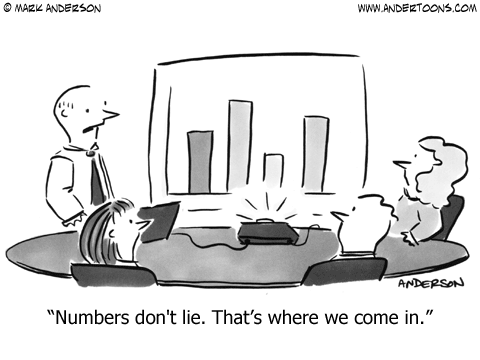
\includegraphics[width=0.5\textwidth,height=\textheight]{images/cartoon3308.png}

\begin{enumerate}
\def\labelenumi{\arabic{enumi}.}
\setcounter{enumi}{2}
\tightlist
\item
  Recognize the importance of data collection, identify limitations in
  data collection methods, and determine how they affect the scope of
  inference.
\item
  Build a conceptual understanding of the unified nature of statistical
  inference.
\item
  Apply estimation and testing methods to analyze single variables or
  the relationship between two variables in order to understand natural
  phenomena and make data-based decisions.
\item
  Model numerical response variables using a single or multiple
  explanatory variables.
\item
  Interpret results in context without relying on statistical jargon.
\item
  Critique and evaluate data-based claims and decisions.
\end{enumerate}

\hypertarget{course-structure}{%
\section*{Course Structure}\label{course-structure}}
\addcontentsline{toc}{section}{Course Structure}

This class will follow an active learning design. Meaning the majority
of each lecture will be dedicated to working on activities. A lot of
what you do in this course will involve writing code, and coding is a
skill that is best learned by doing. A typical class will devote 10-15
minutes to discussion/lecture with the remainder of the class devoted to
working on activities where students will either work by themselves or
in groups. Throughout the class we will discuss and review the work on
the activities. In many cases we may come together to work on parts of
an activity as a class.

\hypertarget{textbooks}{%
\section*{Textbooks}\label{textbooks}}
\addcontentsline{toc}{section}{Textbooks}

We will be using
\href{https://nustat.github.io/intro-stat-ds/}{Introduction to
Statistics and Data Science} which is a free online book that we have
been developing for this course.

\hypertarget{software}{%
\section*{Software}\label{software}}
\addcontentsline{toc}{section}{Software}

We will be using/introducing the free statistical software
\href{https://rstuido.cloud/}{RStudio Cloud}.

\hypertarget{hardware}{%
\section*{Hardware}\label{hardware}}
\addcontentsline{toc}{section}{Hardware}

Students will need a laptop or Chromebook to be able to follow lectures
and to work with RStudio Cloud to complete activities. If access to a
laptop is an issue, then please contact the course instructor and we
will work to find an accommodation.

\hypertarget{assessment}{%
\section*{Assessment}\label{assessment}}
\addcontentsline{toc}{section}{Assessment}

Assessment for the course is comprised of five components:
participation, reading checks, activities, 3 exams, and final project.

\hypertarget{participation}{%
\subsection*{Participation}\label{participation}}
\addcontentsline{toc}{subsection}{Participation}

\hypertarget{reading-checks}{%
\subsection*{Reading Checks}\label{reading-checks}}
\addcontentsline{toc}{subsection}{Reading Checks}

\emph{The lowest three grades will be dropped at the end of the
semester.}

\hypertarget{activities}{%
\subsection*{Activities}\label{activities}}
\addcontentsline{toc}{subsection}{Activities}

\emph{The lowest homework grade will be dropped at the end of the
semester.}

\hypertarget{exams}{%
\subsection*{Exams}\label{exams}}
\addcontentsline{toc}{subsection}{Exams}

The midterm exam will focus on conceptual knowledge of course material
and be taken in-class through the IMathAS software. Students will be
allowed one 8.5 x 11 inch cheat sheet (front \& back) on the in-class
exams.

\hypertarget{final-project}{%
\subsection*{Final Project}\label{final-project}}
\addcontentsline{toc}{subsection}{Final Project}

The projects will focus on practical application of course material.
More information about the project will be provided during the quarter.

\hypertarget{exam-improvement-policy}{%
\subsection*{Exam Improvement Policy}\label{exam-improvement-policy}}
\addcontentsline{toc}{subsection}{Exam Improvement Policy}

We have worked to develop a policy geared towards a growth mindset. That
is, we want a policy where students clearly demonstrate that they have
used the midterm as a diagnostic tool to learn from and improve their
understanding of statistics. Since the final is cumulative we have
settled on a policy where we will replace your in-class midterm score
with your in-class final score --- only in cases where it is an
improvement

\hypertarget{grading}{%
\section*{Grading}\label{grading}}
\addcontentsline{toc}{section}{Grading}

The final course grade will be calculated as follows:

\begin{longtable}[]{@{}ll@{}}
\toprule()
Category & Percentage \\
\midrule()
\endhead
Participation & 5\% \\
Reading Check & 15\% \\
Activities & 10\% \\
Exam 1 & 20\% \\
Exam 2 & 20\% \\
Exam 3 & 20\% \\
Project & 10\% \\
\bottomrule()
\end{longtable}

The final letter grade will be determined based on the following
thresholds:

\begin{longtable}[]{@{}ll@{}}
\toprule()
Letter Grade & Final Grade \\
\midrule()
\endhead
A & \textgreater= 93 \\
A- & 90 - 92.9 \\
B+ & 87 - 89.9 \\
B & 83 - 86.9 \\
B- & 80 - 82.9 \\
C+ & 77 - 79.9 \\
C & 73 - 76.9 \\
C- & 70 - 72.9 \\
D & 60 - 69.9 \\
F & \textless{} 59.9 \\
\bottomrule()
\end{longtable}

\hypertarget{tips-for-success}{%
\section*{Tips for success}\label{tips-for-success}}
\addcontentsline{toc}{section}{Tips for success}

\begin{itemize}
\tightlist
\item
  Dedicate yourself to being an active and engaged learner.
\item
  Prepare for class by \emph{reading and working} through code
  \emph{before} class.
\item
  Work in groups to learn and complete activities.
\item
  Ask questions! Ask them during class, office hours, or on Campuswire.
\item
  Contribute to a welcoming and inclusive learning environment.
\item
  Don't be afraid to make mistakes, you learn from mistakes.
\end{itemize}

\hypertarget{asking-questions-course-communication}{%
\section*{Asking Questions \& Course
Communication}\label{asking-questions-course-communication}}
\addcontentsline{toc}{section}{Asking Questions \& Course Communication}

This term we will be using \href{https://campuswire.com}{Campuswire}
(``Enrollment Code: XXXX'') as our preferred platform for questions
about activities, reading checks, and general course questions. The
system is highly catered to getting you help quickly and efficiently
from classmates and the instructional team. Rather than emailing
questions to the instructional team, you should post your questions on
Campuswire.

The instructional team will check Campuswire periodically and answer
questions, but we strongly encourage students to answer each other's
questions. To this end, student will be able to earn bonus points ---
see Canvas for details.

Please do not expect answers during weekends and evenings.

\hypertarget{school-policies}{%
\section*{School Policies}\label{school-policies}}
\addcontentsline{toc}{section}{School Policies}

Add your standard school policies here.

\bookmarksetup{startatroot}

\hypertarget{tentative-schedule}{%
\chapter*{Tentative schedule}\label{tentative-schedule}}
\addcontentsline{toc}{chapter}{Tentative schedule}

\hypertarget{week-schedule}{%
\section*{11 week Schedule}\label{week-schedule}}
\addcontentsline{toc}{section}{11 week Schedule}

\begin{longtable}[]{@{}
  >{\raggedright\arraybackslash}p{(\columnwidth - 6\tabcolsep) * \real{0.1039}}
  >{\raggedright\arraybackslash}p{(\columnwidth - 6\tabcolsep) * \real{0.4156}}
  >{\raggedright\arraybackslash}p{(\columnwidth - 6\tabcolsep) * \real{0.2987}}
  >{\raggedright\arraybackslash}p{(\columnwidth - 6\tabcolsep) * \real{0.1818}}@{}}
\toprule()
\begin{minipage}[b]{\linewidth}\raggedright
\end{minipage} & \begin{minipage}[b]{\linewidth}\raggedright
Topic
\end{minipage} & \begin{minipage}[b]{\linewidth}\raggedright
Textbook
\end{minipage} & \begin{minipage}[b]{\linewidth}\raggedright
Agenda
\end{minipage} \\
\midrule()
\endhead
Day 1 & Syllabus Day & & Syllabus Day \\
Day 2 & Intro to R & Preface and Chapter 1 & Activity 01 \\
Day 3 & Data Visualization & Sections 2.0-2.3 & Activity 02 \\
Day 4 & Data Visualization & Sections 2.4-2.6 & Activity 03 \\
Day 5 & Data Visualization & Sections 2.7-2.9 & Activity 04 \\
Day 6 & Data Wrangling & Sections 3.0-3.3 & Activity 05 \\
Day 7 & Data Wrangling & Sections 3.4-3.9 & Activity 06 \\
Day 8 & Tidy Data & Chapter 4 & Activity 07 \\
Day 9 & Exam 1 & & \\
Day 10 & Regression & Sections 5.0-5.1 & Activity 08 \\
Day 11 & Regression & Sections 5.2-5.4 & Activity 09 \\
Day 12 & Regression & Sections 6.0-6.1 & Activity 10 \\
Day 13 & Regression & Sections 6.2-6.4 & Activity 11 \\
Day 14 & Randomization + Causality & Chapter 7 & Activity 12 \\
Day 15 & Populations + Generalizability & Chapter 8 & Activity 13 \\
Day 16 & Exam 2 & & \\
Day 17 & Distributions & Sections 9.0-9.1 & Activity 14 \\
Day 18 & Repeated Sampling & Sections 9.2-9.4 & Activity 15 \\
Day 19 & CLT & Sections 9.5-9.7 & Activity 16 \\
Day 20 & Confidence Intervals & Chapter 10 & Activity 17 \\
Day 21 & Confidence Intervals & Chapter 10 & Activity 17 \\
Day 22 & P-values & Chapter 11 & Activity 18 \\
Day 23 & Hypothesis Testing & Chapter 12 & Activity 19 \\
Day 24 & Hypothesis Testing & Chapter 12 & Activity 20 \\
Day 25 & Hypothesis Testing & Chapter 12 & Activity 20 \\
Day 26 & Review & Chapter 13 & \\
Day 27 & Exam 3 & & \\
\bottomrule()
\end{longtable}

\hypertarget{week-schedule-1}{%
\section*{15 week Schedule}\label{week-schedule-1}}
\addcontentsline{toc}{section}{15 week Schedule}

\begin{longtable}[]{@{}
  >{\raggedright\arraybackslash}p{(\columnwidth - 6\tabcolsep) * \real{0.1039}}
  >{\raggedright\arraybackslash}p{(\columnwidth - 6\tabcolsep) * \real{0.4156}}
  >{\raggedright\arraybackslash}p{(\columnwidth - 6\tabcolsep) * \real{0.2987}}
  >{\raggedright\arraybackslash}p{(\columnwidth - 6\tabcolsep) * \real{0.1818}}@{}}
\toprule()
\begin{minipage}[b]{\linewidth}\raggedright
\end{minipage} & \begin{minipage}[b]{\linewidth}\raggedright
Topic
\end{minipage} & \begin{minipage}[b]{\linewidth}\raggedright
Textbook
\end{minipage} & \begin{minipage}[b]{\linewidth}\raggedright
Agenda
\end{minipage} \\
\midrule()
\endhead
Day 1 & Syllabus Day & & Syllabus Day \\
Day 2 & Intro to R & Preface and Chapter 1 & Activity 01 \\
Day 3 & Data Visualization & Sections 2.0-2.3 & Activity 02 \\
Day 4 & Data Visualization & Sections 2.4-2.6 & Activity 03 \\
Day 5 & Data Visualization & Sections 2.7-2.9 & Activity 04 \\
Day 6 & Data Wrangling & Sections 3.0-3.3 & Activity 05 \\
Day 7 & Data Wrangling & Sections 3.4-3.9 & Activity 06 \\
Day 8 & Tidy Data & Chapter 4 & Activity 07 \\
Day 9 & Putting it together & & \\
Day 10 & Review & & \\
Day 11 & Exam 1 & & \\
Day 12 & Regression & Sections 5.0-5.1 & Activity 08 \\
Day 13 & Regression & Sections 5.2-5.4 & Activity 09 \\
Day 14 & Regression & Sections 6.0-6.1 & Activity 10 \\
Day 15 & Regression & Sections 6.2-6.4 & Activity 11 \\
Day 16 & Randomization + Causality & Chapter 7 & Activity 12 \\
Day 17 & Populations + Generalizability & Chapter 8 & Activity 13 \\
Day 18 & Distributions & Sections 9.0-9.1 & Activity 14 \\
Day 19 & Repeated Sampling & Sections 9.2-9.4 & Activity 15 \\
Day 20 & CLT & Sections 9.5-9.7 & Activity 16 \\
Day 21 & Review & & \\
Day 22 & Exam 2 & & \\
Day 23 & Confidence Intervals & Chapter 10 & Activity 17 \\
Day 24 & Confidence Intervals & Chapter 10 & Activity 17 \\
Day 25 & P-values & Chapter 11 & Activity 18 \\
Day 26 & Hypothesis Testing & Chapter 12 & Activity 19 \\
Day 27 & Hypothesis Testing & Chapter 12 & Activity 20 \\
Day 28 & Hypothesis Testing & Chapter 12 & Activity 20 \\
Day 29 & Hypothesis Testing & Chapter 12 & Activity 21 \\
Day 30 & Putting it all together & Chapter 13 & Activity 22 \\
Day 31 & Putting it all together & Chapter 13 & Activity 22 \\
Day 32 & CI - SD & & \\
Day 33 & CI - SD & & \\
Day 34 & Hypothesis - SD & & \\
Day 35 & Hypothesis - SD & & \\
Day 36 & & & \\
Day 37 & & & \\
Day 38 & Review & & \\
Day 39 & Exam 3 & & \\
Day 40 & Project Work Day & & \\
Day 41 & Project Work Day & & \\
Day 42 & Project Work Day & & \\
Day 43 & Project Work Day & & \\
\bottomrule()
\end{longtable}

\bookmarksetup{startatroot}

\hypertarget{day-01}{%
\chapter*{Day 01}\label{day-01}}
\addcontentsline{toc}{chapter}{Day 01}

Welcome to class! Today is all about getting setup with the needed
resources and reviewing the syllabus.

\begin{tcolorbox}[enhanced jigsaw, toptitle=1mm, colback=white, arc=.35mm, rightrule=.15mm, titlerule=0mm, left=2mm, breakable, bottomtitle=1mm, bottomrule=.15mm, leftrule=.75mm, title={Agenda}, colframe=quarto-callout-note-color-frame, opacitybacktitle=0.6, toprule=.15mm, colbacktitle=quarto-callout-note-color!10!white, coltitle=black, opacityback=0]
\textasciitilde{} 15 min Syllabus and expectations.

\textasciitilde{} 20 min Welcome and get students setup with all of the
needed resources.

\textasciitilde{} 15 min Students take survey and get to know their
neighbors.
\end{tcolorbox}

\hypertarget{slide-deck}{%
\section*{Slide Deck}\label{slide-deck}}
\addcontentsline{toc}{section}{Slide Deck}

\begin{tcolorbox}[enhanced jigsaw, toptitle=1mm, colback=white, arc=.35mm, rightrule=.15mm, titlerule=0mm, left=2mm, breakable, bottomtitle=1mm, bottomrule=.15mm, leftrule=.75mm, title={Teaching note:}, colframe=quarto-callout-important-color-frame, opacitybacktitle=0.6, toprule=.15mm, colbacktitle=quarto-callout-important-color!10!white, coltitle=black, opacityback=0]
I recommend using RStudio Cloud if possible for ease of getting started.
Otherwise you will need to dedicate more time towards downloading R and
RStudio. See the sample survey for some examples of questions to ask
your students! We use these survey results on the exams.
\end{tcolorbox}

\begin{tcolorbox}[enhanced jigsaw, breakable, colback=white, bottomrule=.15mm, leftrule=.75mm, colframe=quarto-callout-note-color-frame, arc=.35mm, rightrule=.15mm, toprule=.15mm, left=2mm, opacityback=0]

Make sure you have completed the following agenda items by the end of
class!

\begin{enumerate}
\def\labelenumi{\arabic{enumi}.}
\tightlist
\item
  Review the syllabus
\item
  Visit the course's
  \href{https://campuswire.com/p/G88B46A25}{Campuswire page} using your
  @u.northwestern.edu email. Enrollment code: 7930
\item
  Gain access to the RStudio Cloud Class Workspace (link on Canvas)
\item
  We will be using \href{https://ahaslides.com/202PART1}{AHA slides} for
  participation this quarter.
\item
  Complete the
  \href{https://docs.google.com/forms/d/e/1FAIpQLSfdKddsg7CoaY7WwM2gc9iiUKr8mtSRbKQ8oLAgD9cv0ugJRw/viewform?usp=sf_link}{google
  survey} - we will use this data later.
\item
  Test out the homework system Reading Check 01 (RC 01).
\item
  Login/create your \href{https://northwestern.zoom.us/}{Northwestern
  Zoom Account} if you do not have one. This will be used for office
  hours or requested appointments.
\end{enumerate}

\end{tcolorbox}

\hypertarget{homework}{%
\section*{Homework}\label{homework}}
\addcontentsline{toc}{section}{Homework}

\begin{itemize}
\item
  Read Preface and Chapter 1 of the book
\item
  Complete and submit Reading Check 01\_intro
\end{itemize}

\bookmarksetup{startatroot}

\hypertarget{day-02}{%
\chapter*{Day 02}\label{day-02}}
\addcontentsline{toc}{chapter}{Day 02}

Today's lesson covers
\href{https://nustat.github.io/intro-stat-data-sci/}{Preface and Chapter
1} and focuses on students getting familiar with Quarto in RStudio.

\begin{tcolorbox}[enhanced jigsaw, toptitle=1mm, colback=white, arc=.35mm, rightrule=.15mm, titlerule=0mm, left=2mm, breakable, bottomtitle=1mm, bottomrule=.15mm, leftrule=.75mm, title={Agenda}, colframe=quarto-callout-note-color-frame, opacitybacktitle=0.6, toprule=.15mm, colbacktitle=quarto-callout-note-color!10!white, coltitle=black, opacityback=0]
\textasciitilde{} 25 min Students work in groups or independently on
Activity 01.

\textasciitilde{} 20 min Thoroughly walk through and discuss Activity 01
as a class.

\textasciitilde{} ~ 5 min Make sure students know how to submit their
activity! ~~ Go through Slide Deck 01.
\end{tcolorbox}

\hypertarget{activity-solution}{%
\section*{Activity Solution}\label{activity-solution}}
\addcontentsline{toc}{section}{Activity Solution}

\begin{tcolorbox}[enhanced jigsaw, toptitle=1mm, colback=white, arc=.35mm, rightrule=.15mm, titlerule=0mm, left=2mm, breakable, bottomtitle=1mm, bottomrule=.15mm, leftrule=.75mm, title={Task 2}, colframe=quarto-callout-important-color-frame, opacitybacktitle=0.6, toprule=.15mm, colbacktitle=quarto-callout-important-color!10!white, coltitle=black, opacityback=0]
title: ``Quarto Practice'' subtitle: ``Activity 01'' author: ``Willie
Wildcat'' date: ``2022-09-23'' format: html
\end{tcolorbox}

\hypertarget{quarto}{%
\subsection*{Quarto}\label{quarto}}
\addcontentsline{toc}{subsection}{Quarto}

Quarto enables you to weave together content and executable code into a
finished document. To learn more about Quarto see
\url{https://quarto.org}.

\begin{tcolorbox}[enhanced jigsaw, toptitle=1mm, colback=white, arc=.35mm, rightrule=.15mm, titlerule=0mm, left=2mm, breakable, bottomtitle=1mm, bottomrule=.15mm, leftrule=.75mm, title={Task 6 (message: false is `Challenge')}, colframe=quarto-callout-important-color-frame, opacitybacktitle=0.6, toprule=.15mm, colbacktitle=quarto-callout-important-color!10!white, coltitle=black, opacityback=0]

\hypertarget{loading-package}{%
\subsection*{Loading Package}\label{loading-package}}
\addcontentsline{toc}{subsection}{Loading Package}

\begin{Shaded}
\begin{Highlighting}[]
\InformationTok{\textasciigrave{}\textasciigrave{}\textasciigrave{}\{r\}}
\CommentTok{\#| label: load{-}pkgs}
\CommentTok{\#| message: false}
\FunctionTok{library}\NormalTok{(nycflights13)}
\FunctionTok{library}\NormalTok{(dplyr)}
\FunctionTok{library}\NormalTok{(knitr)}
\InformationTok{\textasciigrave{}\textasciigrave{}\textasciigrave{}}
\end{Highlighting}
\end{Shaded}

\end{tcolorbox}

\hypertarget{running-code}{%
\subsection*{Running Code}\label{running-code}}
\addcontentsline{toc}{subsection}{Running Code}

When you click the \textbf{Render} button a document will be generated
that includes both content and the output of embedded code. You can
embed code like this:

\begin{Shaded}
\begin{Highlighting}[]
\InformationTok{\textasciigrave{}\textasciigrave{}\textasciigrave{}\{r\}}

\DecValTok{1} \SpecialCharTok{+} \DecValTok{1}
\InformationTok{\textasciigrave{}\textasciigrave{}\textasciigrave{}}
\end{Highlighting}
\end{Shaded}

\begin{verbatim}
[1] 2
\end{verbatim}

You can add options to executable code like this

\begin{verbatim}
[1] 4
\end{verbatim}

The \texttt{echo:\ false} option disables the printing of code (only
output is displayed).

\hypertarget{tasks}{%
\subsection*{Tasks}\label{tasks}}
\addcontentsline{toc}{subsection}{Tasks}

Complete the following series of tasks. Remember to \textbf{render early
and render often}.

\hypertarget{task-1}{%
\subsubsection*{Task 1}\label{task-1}}
\addcontentsline{toc}{subsubsection}{Task 1}

It will be easier for you to compare your qmd file to the html file if
we make a slight change to the RStudio settings.

\begin{itemize}
\tightlist
\item
  Find the gear/sprocket icon next to the \textbf{Render} button.
\item
  Click it and then select \textbf{Preview in Viewer Pane}.
\item
  Render the document to see the change.
\end{itemize}

Now take some time to compare what you see in this document with the
html version that is now previewed in the viewer pane.

\hypertarget{task-2-1}{%
\subsubsection*{Task 2}\label{task-2-1}}
\addcontentsline{toc}{subsubsection}{Task 2}

Let's make some adjustments to the document:

\begin{enumerate}
\def\labelenumi{\arabic{enumi}.}
\tightlist
\item
  Change the title to ``Quarto Practice''.
\item
  Add an ``Activity 01'' as a subtitle. Hint \texttt{subtitle:} goes
  right below \texttt{title:}.
\item
  Change the author to your name.
\item
  Change the date to today's date in ``YYYY-MM-DD'' format. Example
  9/1/2030 becomes 2030-09-01.
\end{enumerate}

\hypertarget{task-3}{%
\subsubsection*{Task 3}\label{task-3}}
\addcontentsline{toc}{subsubsection}{Task 3}

Insert an R code chunk BELOW and name it \texttt{task3}. Place the
following two lines of code in it:

\begin{tcolorbox}[enhanced jigsaw, breakable, colback=white, bottomrule=.15mm, leftrule=.75mm, colframe=quarto-callout-important-color-frame, arc=.35mm, rightrule=.15mm, toprule=.15mm, left=2mm, opacityback=0]

\begin{Shaded}
\begin{Highlighting}[]
\InformationTok{\textasciigrave{}\textasciigrave{}\textasciigrave{}\{r\}}
\CommentTok{\#| label: task3}
\NormalTok{x }\OtherTok{\textless{}{-}} \DecValTok{9}
\NormalTok{y }\OtherTok{\textless{}{-}} \DecValTok{45}
\InformationTok{\textasciigrave{}\textasciigrave{}\textasciigrave{}}
\end{Highlighting}
\end{Shaded}

\end{tcolorbox}

The \texttt{\textless{}-} is an assignment operator. Here it assigned
the number 9 to \texttt{x} and the number 45 to y. You store values so
that you can access them by name later!

\hypertarget{task-4}{%
\subsubsection*{Task 4}\label{task-4}}
\addcontentsline{toc}{subsubsection}{Task 4}

Change the R code chunk options below to \texttt{eval=true} or
alternatively you can simply remove \texttt{\#\textbar{}\ eval=false}
from the code chunk options. Either will have the same effect. This
depends on completing \textbf{Task 3} correctly.

\begin{tcolorbox}[enhanced jigsaw, breakable, colback=white, bottomrule=.15mm, leftrule=.75mm, colframe=quarto-callout-important-color-frame, arc=.35mm, rightrule=.15mm, toprule=.15mm, left=2mm, opacityback=0]
eval: false -\textgreater{} eval: true
\end{tcolorbox}

\begin{Shaded}
\begin{Highlighting}[]
\InformationTok{\textasciigrave{}\textasciigrave{}\textasciigrave{}\{r\}}
\CommentTok{\#| label: task 4}
\CommentTok{\#| eval: true}
\NormalTok{x }\SpecialCharTok{*}\NormalTok{ y}
\InformationTok{\textasciigrave{}\textasciigrave{}\textasciigrave{}}
\end{Highlighting}
\end{Shaded}

\begin{verbatim}
[1] 405
\end{verbatim}

\hypertarget{task-5}{%
\subsubsection*{Task 5}\label{task-5}}
\addcontentsline{toc}{subsubsection}{Task 5}

Let's focus on R code chunks. You may have noticed a down arrow and a
green arrow on the upper right side of the code chunk.

Click the green arrow on the \texttt{task4} R code chunk.

An error MIGHT pop up right below the R chunk (if you did not get an
error that is OKAY - you are one step ahead of us).

Before we address the potential error let's change an RStudio setting.
Again, find the gear/sprocket next to the \textbf{Knit} button. Click it
and select \textbf{Chunk Output in Console}. A pop-up should appear,
select remove output. Now click the green arrow on the \texttt{task4} R
code chunk. Any ouput or message should now appear in the console below.

Now let's take care of the error. Note that the error doesn't appear
when you knit the document. All the code works fine. Test this out if
you haven't already. This seems a little strange?

It comes down to what happens when you click \textbf{Render}. A brand
new session of R is started in the background (you don't see this), it
produces the document, and then closes down.

When we click the green arrow on the \texttt{task4} R code chunk we are
not knitting. We are running code in our \emph{current} R session. If
you never ran the \texttt{task3} code chunk in our \emph{current} R
session the required variables do not exist yet and cannot be used. So
we just need to run the \texttt{task3} code chunk before running the
\texttt{task4} chunk.

Stop for a second and imagine if the \texttt{task4} chunk depended on
several code chunks. We can run all previous code chunks by clicking the
icon with a down arrow and a green bar --- do this for the
\texttt{task4} R code chunk. If you check your environment pane
(top-right), then you will see the needed pieces have been created. Now
click the green arrow on the \texttt{task4} chunk and it should return
\texttt{405} in the console.

\hypertarget{task-6}{%
\subsubsection*{Task 6}\label{task-6}}
\addcontentsline{toc}{subsubsection}{Task 6}

Place a new section right before the \textbf{Running Code} with the
header \textbf{Loading Packages}. Create an R code chunk named
\texttt{load-pkgs} in the section and use it to load
\texttt{nycflights13}, \texttt{dplyr} and \texttt{knitr}.

Now alter the R code chunk below to get it to evaluate/run.

\begin{tcolorbox}[enhanced jigsaw, breakable, colback=white, bottomrule=.15mm, leftrule=.75mm, colframe=quarto-callout-important-color-frame, arc=.35mm, rightrule=.15mm, toprule=.15mm, left=2mm, opacityback=0]
eval: false -\textgreater{} eval: true
\end{tcolorbox}

\begin{Shaded}
\begin{Highlighting}[]
\InformationTok{\textasciigrave{}\textasciigrave{}\textasciigrave{}\{r\}}
\CommentTok{\#| label: kable{-}test}
\CommentTok{\#| eval: true}
\CommentTok{\#| message: false}

\NormalTok{airlines}
\FunctionTok{kable}\NormalTok{(airlines)}
\InformationTok{\textasciigrave{}\textasciigrave{}\textasciigrave{}}
\end{Highlighting}
\end{Shaded}

\begin{verbatim}
# A tibble: 16 x 2
   carrier name                       
   <chr>   <chr>                      
 1 9E      Endeavor Air Inc.          
 2 AA      American Airlines Inc.     
 3 AS      Alaska Airlines Inc.       
 4 B6      JetBlue Airways            
 5 DL      Delta Air Lines Inc.       
 6 EV      ExpressJet Airlines Inc.   
 7 F9      Frontier Airlines Inc.     
 8 FL      AirTran Airways Corporation
 9 HA      Hawaiian Airlines Inc.     
10 MQ      Envoy Air                  
11 OO      SkyWest Airlines Inc.      
12 UA      United Air Lines Inc.      
13 US      US Airways Inc.            
14 VX      Virgin America             
15 WN      Southwest Airlines Co.     
16 YV      Mesa Airlines Inc.         
\end{verbatim}

\begin{longtable}[]{@{}ll@{}}
\toprule()
carrier & name \\
\midrule()
\endhead
9E & Endeavor Air Inc. \\
AA & American Airlines Inc. \\
AS & Alaska Airlines Inc. \\
B6 & JetBlue Airways \\
DL & Delta Air Lines Inc. \\
EV & ExpressJet Airlines Inc. \\
F9 & Frontier Airlines Inc. \\
FL & AirTran Airways Corporation \\
HA & Hawaiian Airlines Inc. \\
MQ & Envoy Air \\
OO & SkyWest Airlines Inc. \\
UA & United Air Lines Inc. \\
US & US Airways Inc. \\
VX & Virgin America \\
WN & Southwest Airlines Co. \\
YV & Mesa Airlines Inc. \\
\bottomrule()
\end{longtable}

\hypertarget{optional-challenge-dont-have-to-complete}{%
\subsubsection*{Optional challenge (don't have to
complete)}\label{optional-challenge-dont-have-to-complete}}
\addcontentsline{toc}{subsubsection}{Optional challenge (don't have to
complete)}

Alter the R code chunk options for \texttt{load-pkgs} to suppress the
\texttt{message}s from appearing.

\hypertarget{task-7}{%
\subsubsection*{Task 7}\label{task-7}}
\addcontentsline{toc}{subsubsection}{Task 7}

\begin{tcolorbox}[enhanced jigsaw, toptitle=1mm, colback=white, arc=.35mm, rightrule=.15mm, titlerule=0mm, left=2mm, breakable, bottomtitle=1mm, bottomrule=.15mm, leftrule=.75mm, title={Teaching note:}, colframe=quarto-callout-important-color-frame, opacitybacktitle=0.6, toprule=.15mm, colbacktitle=quarto-callout-important-color!10!white, coltitle=black, opacityback=0]
Make sure you do this together before the end of class!
\end{tcolorbox}

Export your completed document and submit the activity on Canvas.

\begin{enumerate}
\def\labelenumi{\arabic{enumi}.}
\tightlist
\item
  Be sure you \textbf{always render the final document before} you
  export.
\item
  It will create a document in the \texttt{Files} pane called
  \texttt{Last\_First\_act\_01.html}. Check/click the box next to this
  file.
\item
  In the \texttt{Files} pane navigate to the gear sprocket. And click
  the \texttt{Export...} option.
\item
  Once your .html is downloaded. Look at it BEFORE submitting! Make sure
  everything is completed.
\item
  In Canvas click on the Assignment \texttt{Activity\ 01} and upload the
  html you downloaded.
\end{enumerate}

\hypertarget{slide-deck-1}{%
\section*{Slide Deck}\label{slide-deck-1}}
\addcontentsline{toc}{section}{Slide Deck}

Today's slide deck is more of a resource for student's to refer back to
rather than an actual lecture.

\begin{tcolorbox}[enhanced jigsaw, breakable, colback=white, bottomrule=.15mm, leftrule=.75mm, colframe=quarto-callout-note-color-frame, arc=.35mm, rightrule=.15mm, toprule=.15mm, left=2mm, opacityback=0]

\begin{cols}

\begin{col}{0.6\textwidth}

\begin{enumerate}
\def\labelenumi{\arabic{enumi}.}
\tightlist
\item
  Change the \texttt{yaml} heading on a document
\item
  Create your first code chunk!
\item
  Learn the code chunk settings
\item
  Assign values to a variable
\end{enumerate}

\end{col}

\begin{col}{0.4\textwidth}

\includegraphics[width=\textwidth,height=1in]{images/images_horst/horst_rstudio_air.png}

Artwork by @allison\_horst

\end{col}

\end{cols}

\end{tcolorbox}

\begin{tcolorbox}[enhanced jigsaw, breakable, colback=white, bottomrule=.15mm, leftrule=.75mm, colframe=quarto-callout-note-color-frame, arc=.35mm, rightrule=.15mm, toprule=.15mm, left=2mm, opacityback=0]

\begin{itemize}
\item
  Complete today's activity first!
\item
  These slides just include helpful reminders that you may find useful
  to refer back to when working on later activities.
\end{itemize}

\end{tcolorbox}

\begin{tcolorbox}[enhanced jigsaw, breakable, colback=white, bottomrule=.15mm, leftrule=.75mm, colframe=quarto-callout-note-color-frame, arc=.35mm, rightrule=.15mm, toprule=.15mm, left=2mm, opacityback=0]

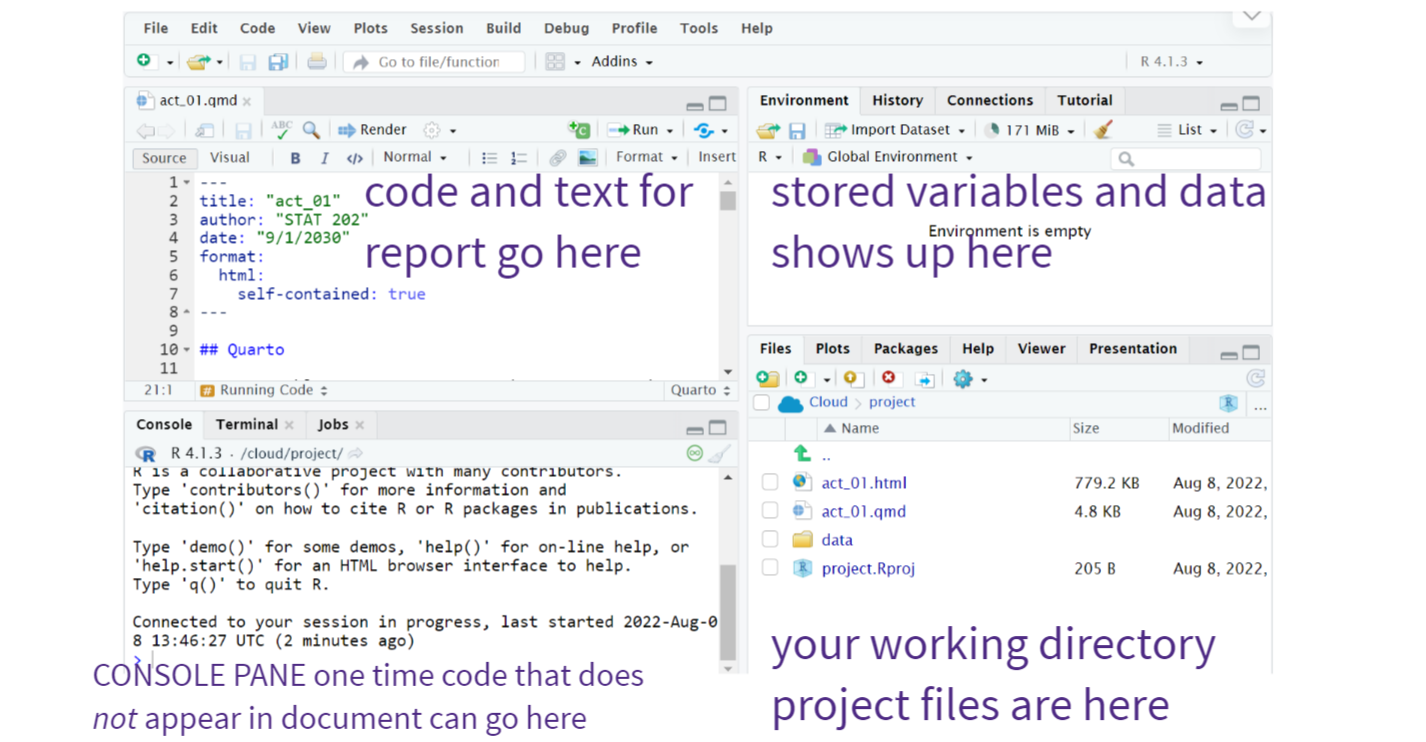
\includegraphics{images/images_guide/rstudio_interface_complete.png}

\end{tcolorbox}

\begin{tcolorbox}[enhanced jigsaw, breakable, colback=white, bottomrule=.15mm, leftrule=.75mm, colframe=quarto-callout-note-color-frame, arc=.35mm, rightrule=.15mm, toprule=.15mm, left=2mm, opacityback=0]

\begin{cols}

\begin{col}{0.5\textwidth}
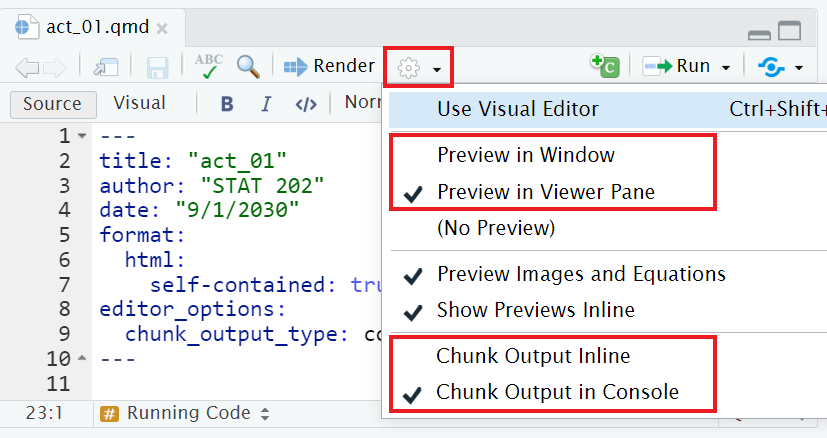
\includegraphics{images/images_lecture/rstudio_viewer.png}

\end{col}

\begin{col}{0.5\textwidth}
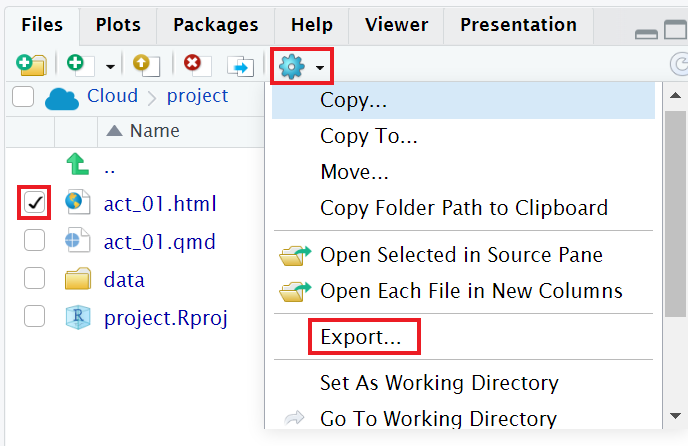
\includegraphics{images/images_lecture/rstudio_export.png}

\end{col}

\end{cols}

\end{tcolorbox}

\begin{tcolorbox}[enhanced jigsaw, breakable, colback=white, bottomrule=.15mm, leftrule=.75mm, colframe=quarto-callout-note-color-frame, arc=.35mm, rightrule=.15mm, toprule=.15mm, left=2mm, opacityback=0]

\begin{cols}

\begin{col}{0.35\textwidth}

\begin{Shaded}
\begin{Highlighting}[]
\InformationTok{\textasciigrave{}\textasciigrave{}\textasciigrave{}\{r\}}
\CommentTok{\#| message: false}
\CommentTok{\#| warning: false}
\CommentTok{\#| eval: false}
\CommentTok{\#| echo: false}
\CommentTok{\#| include: false}
\InformationTok{\textasciigrave{}\textasciigrave{}\textasciigrave{}}
\end{Highlighting}
\end{Shaded}

\end{col}

\begin{col}{0.65\textwidth}

\begin{itemize}
\item
  \texttt{message:\ false} prevents messages from appearing in knitted
  doc
\item
  \texttt{warning:\ false} prevents warnings from appearing in knitted
  doc
\item
  \texttt{eval:\ false} includes the code chunk in the knitted document
  but prevents the code chunk from being run
\item
  \texttt{echo:\ false} prevents code itself from printing but includes
  the results of the code
\item
  \texttt{include:\ false} prevents code and its results from printing
  but still runs the code when knitted
\end{itemize}

\end{col}

\end{cols}

\end{tcolorbox}

\hypertarget{homework-1}{%
\section*{Homework}\label{homework-1}}
\addcontentsline{toc}{section}{Homework}

\begin{itemize}
\item
  Complete and submit Activity 01
\item
  Read Sections 2.0 - 2.3 of the book
\item
  Complete and submit Reading Check 02\_ggplot1
\end{itemize}

\bookmarksetup{startatroot}

\hypertarget{day-03}{%
\chapter*{Day 03}\label{day-03}}
\addcontentsline{toc}{chapter}{Day 03}

Onto the real fun now! Today's lesson covers
\href{https://nustat.github.io/intro-stat-data-sci/02-visualization.html}{Section
2.0 - 2.3} and focuses on making scatterplots with \texttt{ggplot()}.

\begin{tcolorbox}[enhanced jigsaw, toptitle=1mm, colback=white, arc=.35mm, rightrule=.15mm, titlerule=0mm, left=2mm, breakable, bottomtitle=1mm, bottomrule=.15mm, leftrule=.75mm, title={Agenda}, colframe=quarto-callout-note-color-frame, opacitybacktitle=0.6, toprule=.15mm, colbacktitle=quarto-callout-note-color!10!white, coltitle=black, opacityback=0]
\textasciitilde{} 15 min Slide deck

\textasciitilde{} 25 min Students work on Activity 02

\textasciitilde{} 10 min Work through a select problem in detail from
the activity as a class
\end{tcolorbox}

\hypertarget{slide-deck-2}{%
\section*{Slide Deck}\label{slide-deck-2}}
\addcontentsline{toc}{section}{Slide Deck}

\begin{tcolorbox}[enhanced jigsaw, breakable, colback=white, bottomrule=.15mm, leftrule=.75mm, colframe=quarto-callout-note-color-frame, arc=.35mm, rightrule=.15mm, toprule=.15mm, left=2mm, opacityback=0]

\begin{cols}

\begin{col}{0.60\textwidth}

\begin{enumerate}
\def\labelenumi{\arabic{enumi}.}
\tightlist
\item
  Create a scatterplot
\item
  Properly describe a scatterplot
\item
  Change aesthetics such as color and shape in your plot
\item
  Solve overplotting issues
\end{enumerate}

\end{col}

\begin{col}{0.40\textwidth}
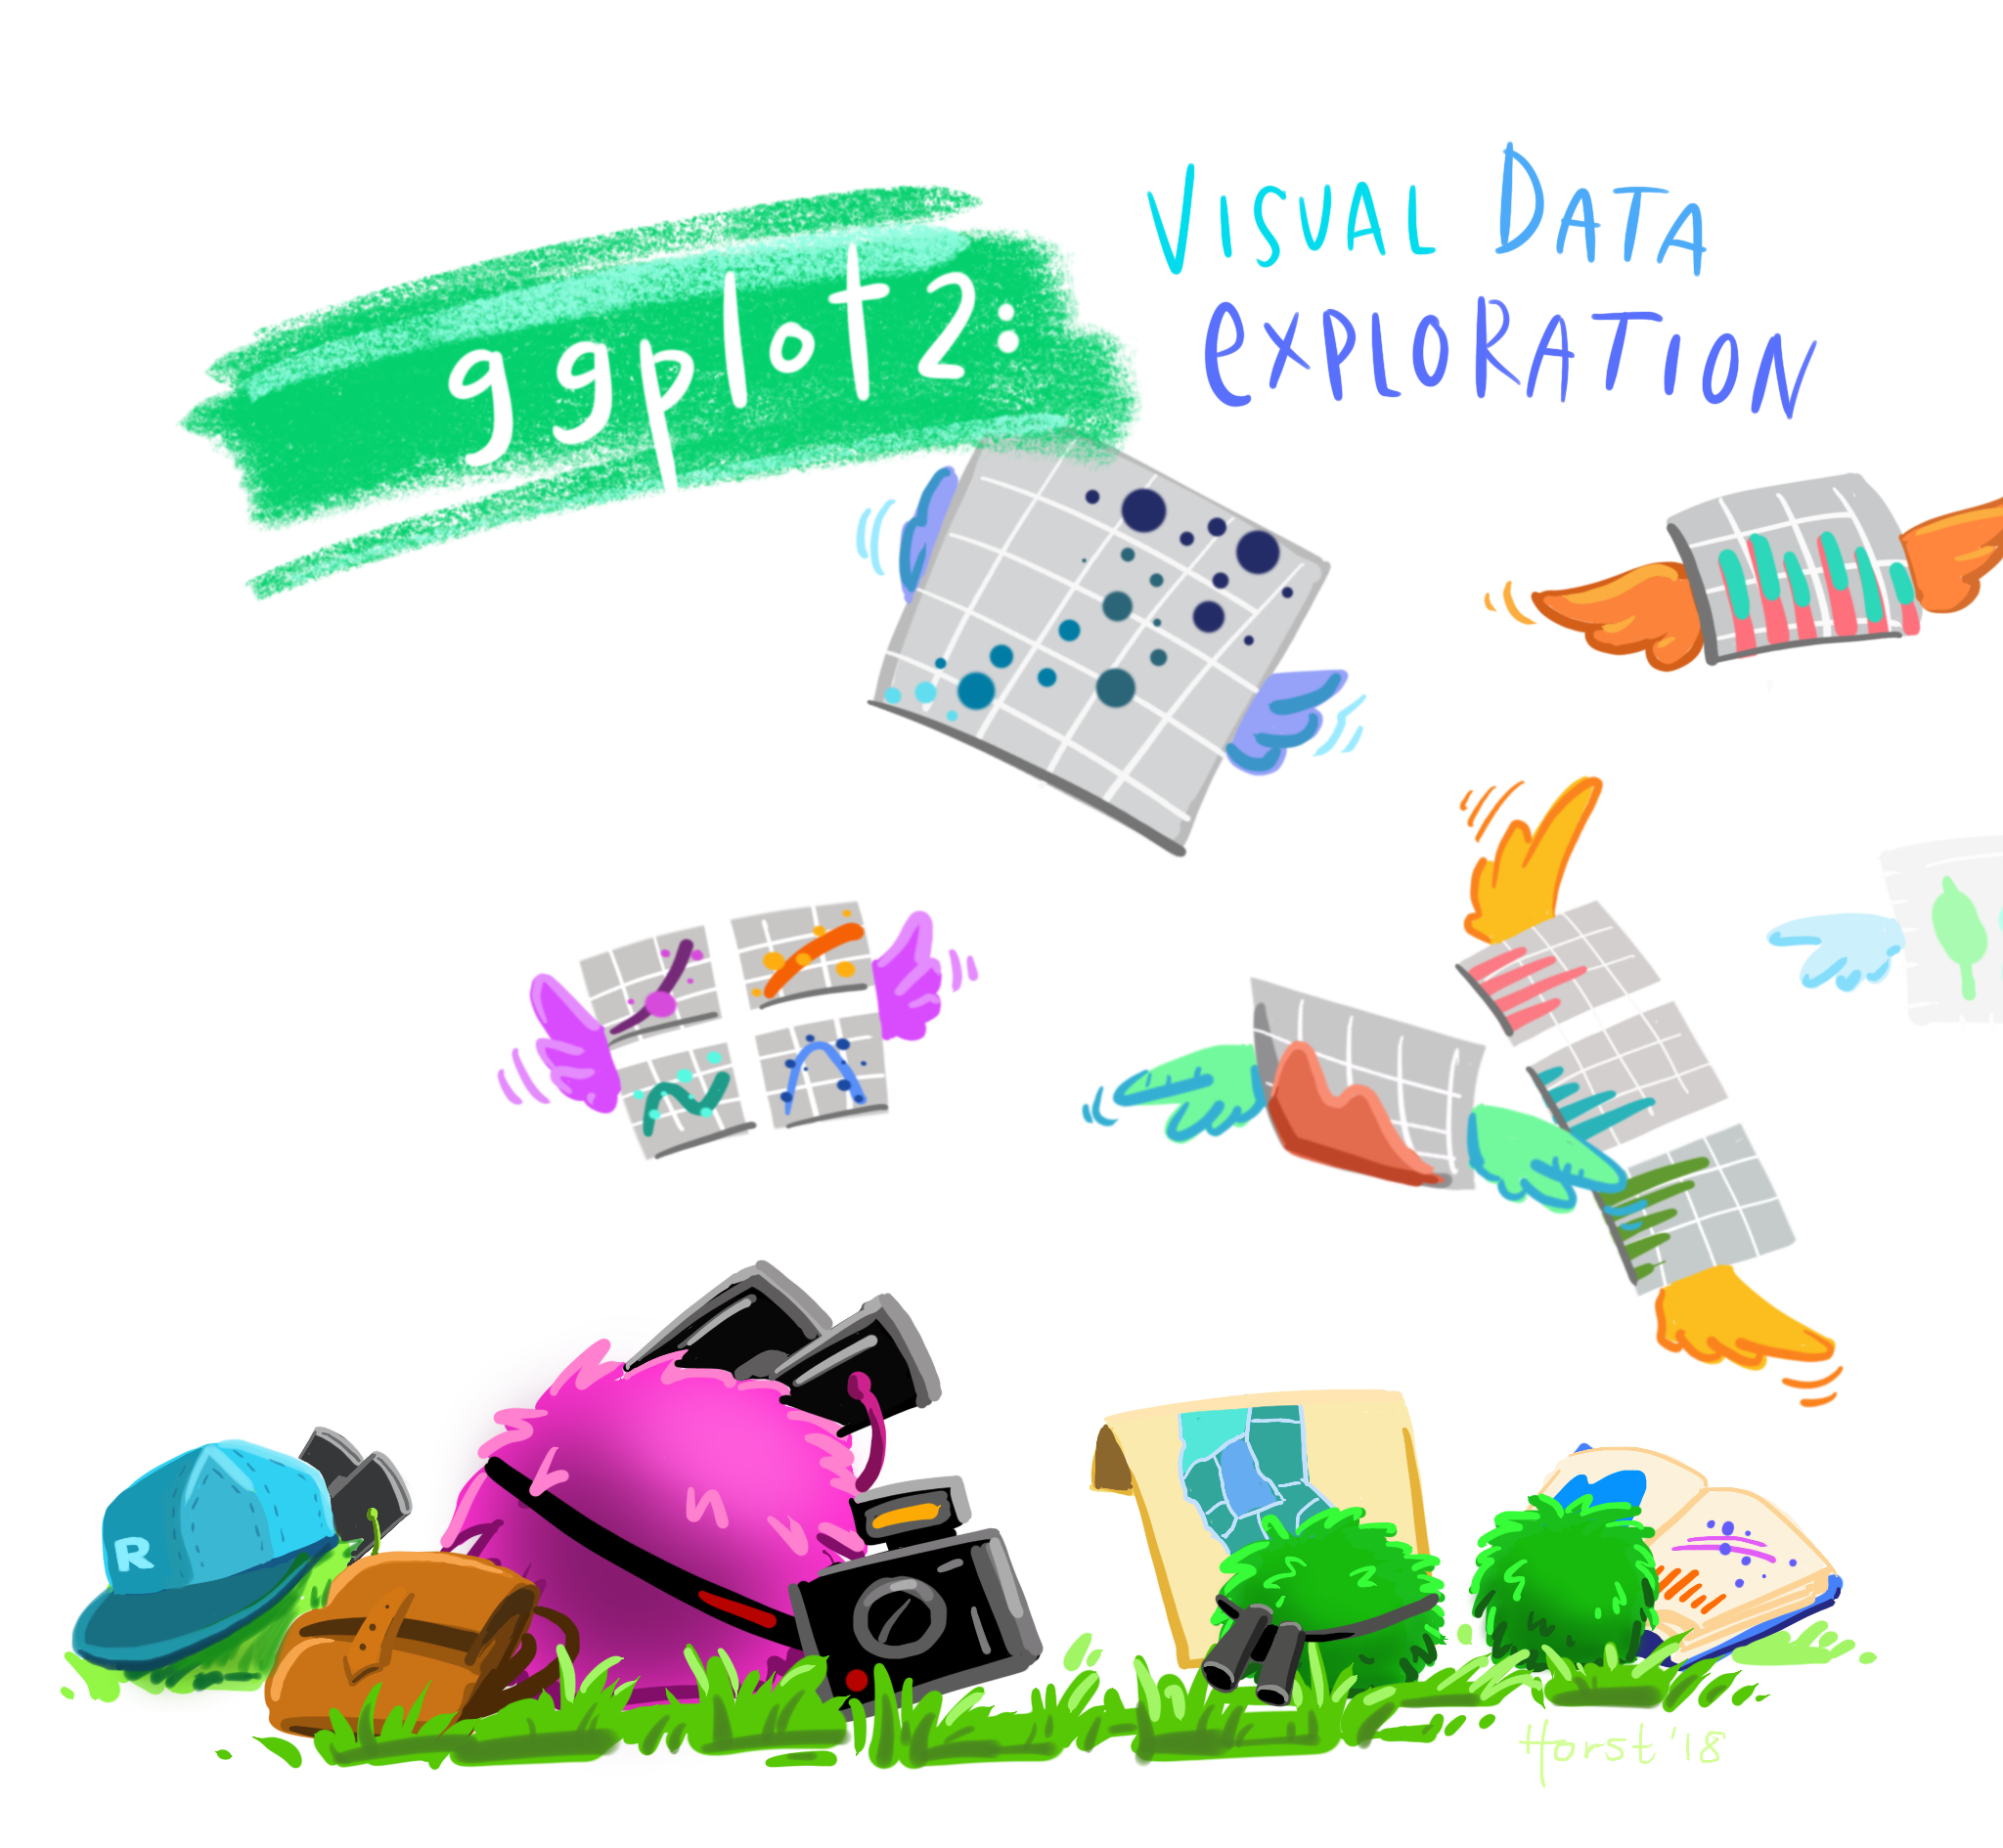
\includegraphics[width=\textwidth,height=1in]{images/images_horst/ggplot2_exploratory.png}
Artwork by @allison\_horst

\end{col}

\end{cols}

\end{tcolorbox}

\begin{tcolorbox}[enhanced jigsaw, breakable, colback=white, bottomrule=.15mm, leftrule=.75mm, colframe=quarto-callout-note-color-frame, arc=.35mm, rightrule=.15mm, toprule=.15mm, left=2mm, opacityback=0]

\begin{cols}

\begin{col}{0.85\textwidth}
Defines a set of rules for constructing statistical graphics by
combining different types of \textbf{layers}.

\end{col}

\begin{col}{0.15\textwidth}
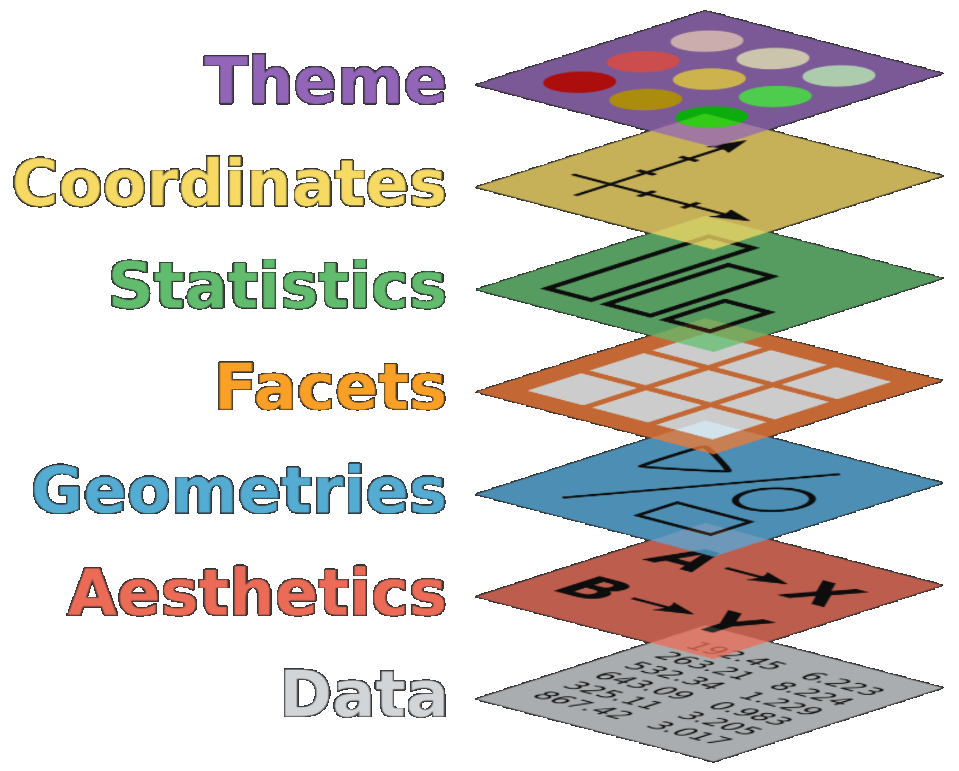
\includegraphics[width=1.04167in,height=1.04167in]{images/images_lecture/grammar_graphics.png}

\end{col}

\end{cols}

\begin{longtable}{lll}
\toprule
Layer & Function & Explanation \\ 
\midrule
Data & ggplot( ) & initialize plot and define dataset first \\ 
Aesthetics & aes( ) & how variables are mapped \\ 
Geometries & geom\_*( ) & how data is conveyed \\ 
Facets & facet\_*( ) & separates plots by categories \\ 
Statistics & stat\_*( ) & statistical transformations \\ 
Coordinates & coord\_*( ) & customize coord system \\ 
Theme & theme( ) & customize non-data components \\ 
\bottomrule
\end{longtable}

Only the \emph{first three} layers are essential components that must be
defined when building a graphic.

\end{tcolorbox}

\begin{tcolorbox}[enhanced jigsaw, breakable, colback=white, bottomrule=.15mm, leftrule=.75mm, colframe=quarto-callout-note-color-frame, arc=.35mm, rightrule=.15mm, toprule=.15mm, left=2mm, opacityback=0]
Scatterplots allow you to visualize the \textbf{relationship} between 2
\textbf{numerical} variables.

\textbf{Scatterplot syntax in R:}

\begin{Shaded}
\begin{Highlighting}[]
\FunctionTok{ggplot}\NormalTok{(}\AttributeTok{data=}\NormalTok{ my\_data, }\AttributeTok{mapping =} \FunctionTok{aes}\NormalTok{(}\AttributeTok{x =}\NormalTok{ var1, }\AttributeTok{y =}\NormalTok{ var2)) }\SpecialCharTok{+}
  \FunctionTok{geom\_point}\NormalTok{()}
\end{Highlighting}
\end{Shaded}

\textbf{Scatterplot language:} Construct a scatterplot of \textbf{Y by
X}.
\end{tcolorbox}

\begin{tcolorbox}[enhanced jigsaw, breakable, colback=white, bottomrule=.15mm, leftrule=.75mm, colframe=quarto-callout-note-color-frame, arc=.35mm, rightrule=.15mm, toprule=.15mm, left=2mm, opacityback=0]

When describing scatterplots\ldots{}

\begin{itemize}
\tightlist
\item
  Look for pattern going from left to right.
\item
  Classify association as positive, negative, or no association.
\item
  Classify strength of association: strong, moderate, weak.
\item
  Describe overall pattern: linear, nonlinear, etc.
\item
  Check for overplotting issues.
\end{itemize}

\end{tcolorbox}

\begin{tcolorbox}[enhanced jigsaw, breakable, colback=white, bottomrule=.15mm, leftrule=.75mm, colframe=quarto-callout-note-color-frame, arc=.35mm, rightrule=.15mm, toprule=.15mm, left=2mm, opacityback=0]

\begin{Shaded}
\begin{Highlighting}[]
\InformationTok{\textasciigrave{}\textasciigrave{}\textasciigrave{}\{r\}}

\FunctionTok{library}\NormalTok{(palmerpenguins)}
\FunctionTok{glimpse}\NormalTok{(penguins)}
\InformationTok{\textasciigrave{}\textasciigrave{}\textasciigrave{}}
\end{Highlighting}
\end{Shaded}

\begin{verbatim}
Rows: 344
Columns: 8
$ species           <fct> Adelie, Adelie, Adelie, Adelie, Adelie, Adelie, Adel~
$ island            <fct> Torgersen, Torgersen, Torgersen, Torgersen, Torgerse~
$ bill_length_mm    <dbl> 39.1, 39.5, 40.3, NA, 36.7, 39.3, 38.9, 39.2, 34.1, ~
$ bill_depth_mm     <dbl> 18.7, 17.4, 18.0, NA, 19.3, 20.6, 17.8, 19.6, 18.1, ~
$ flipper_length_mm <int> 181, 186, 195, NA, 193, 190, 181, 195, 193, 190, 186~
$ body_mass_g       <int> 3750, 3800, 3250, NA, 3450, 3650, 3625, 4675, 3475, ~
$ sex               <fct> male, female, female, NA, female, male, female, male~
$ year              <int> 2007, 2007, 2007, 2007, 2007, 2007, 2007, 2007, 2007~
\end{verbatim}

\begin{cols}

\begin{col}{0.5\textwidth}
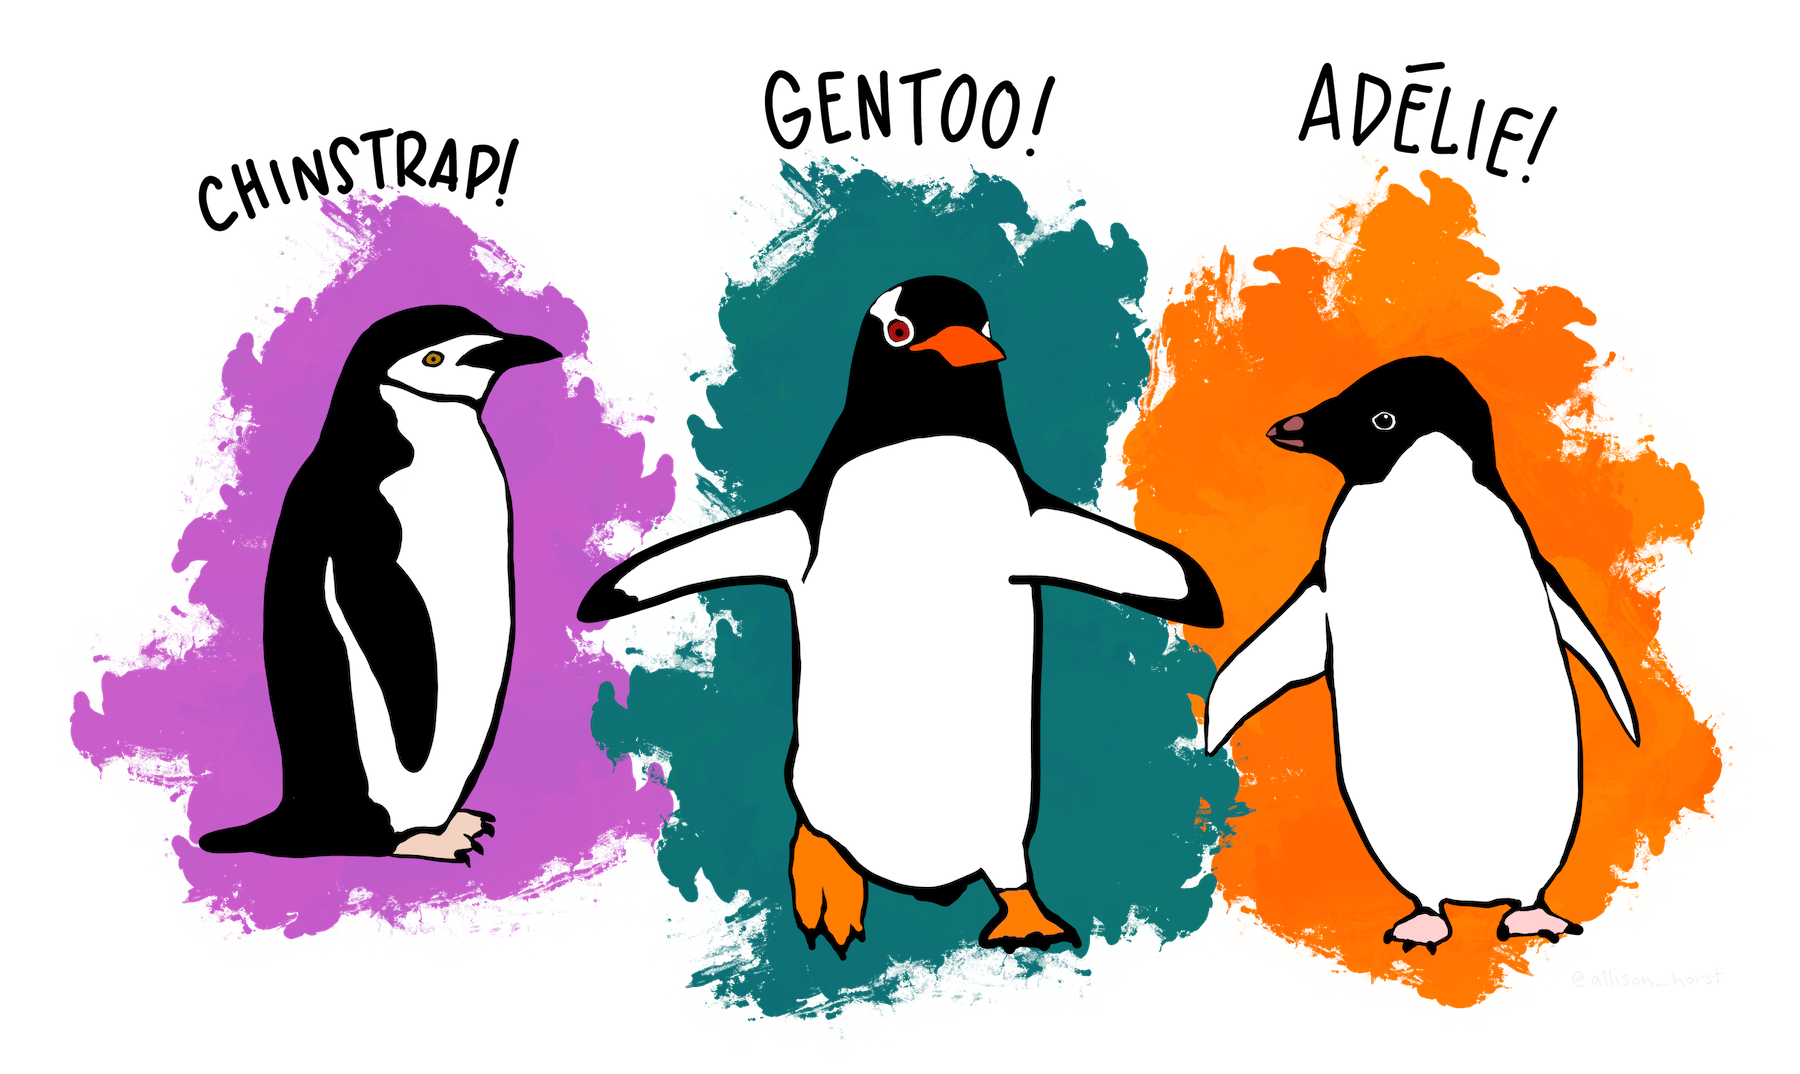
\includegraphics[width=2.08333in,height=1.5625in]{images/images_horst/palmer_penguin_species.png}

\end{col}

\begin{col}{0.5\textwidth}
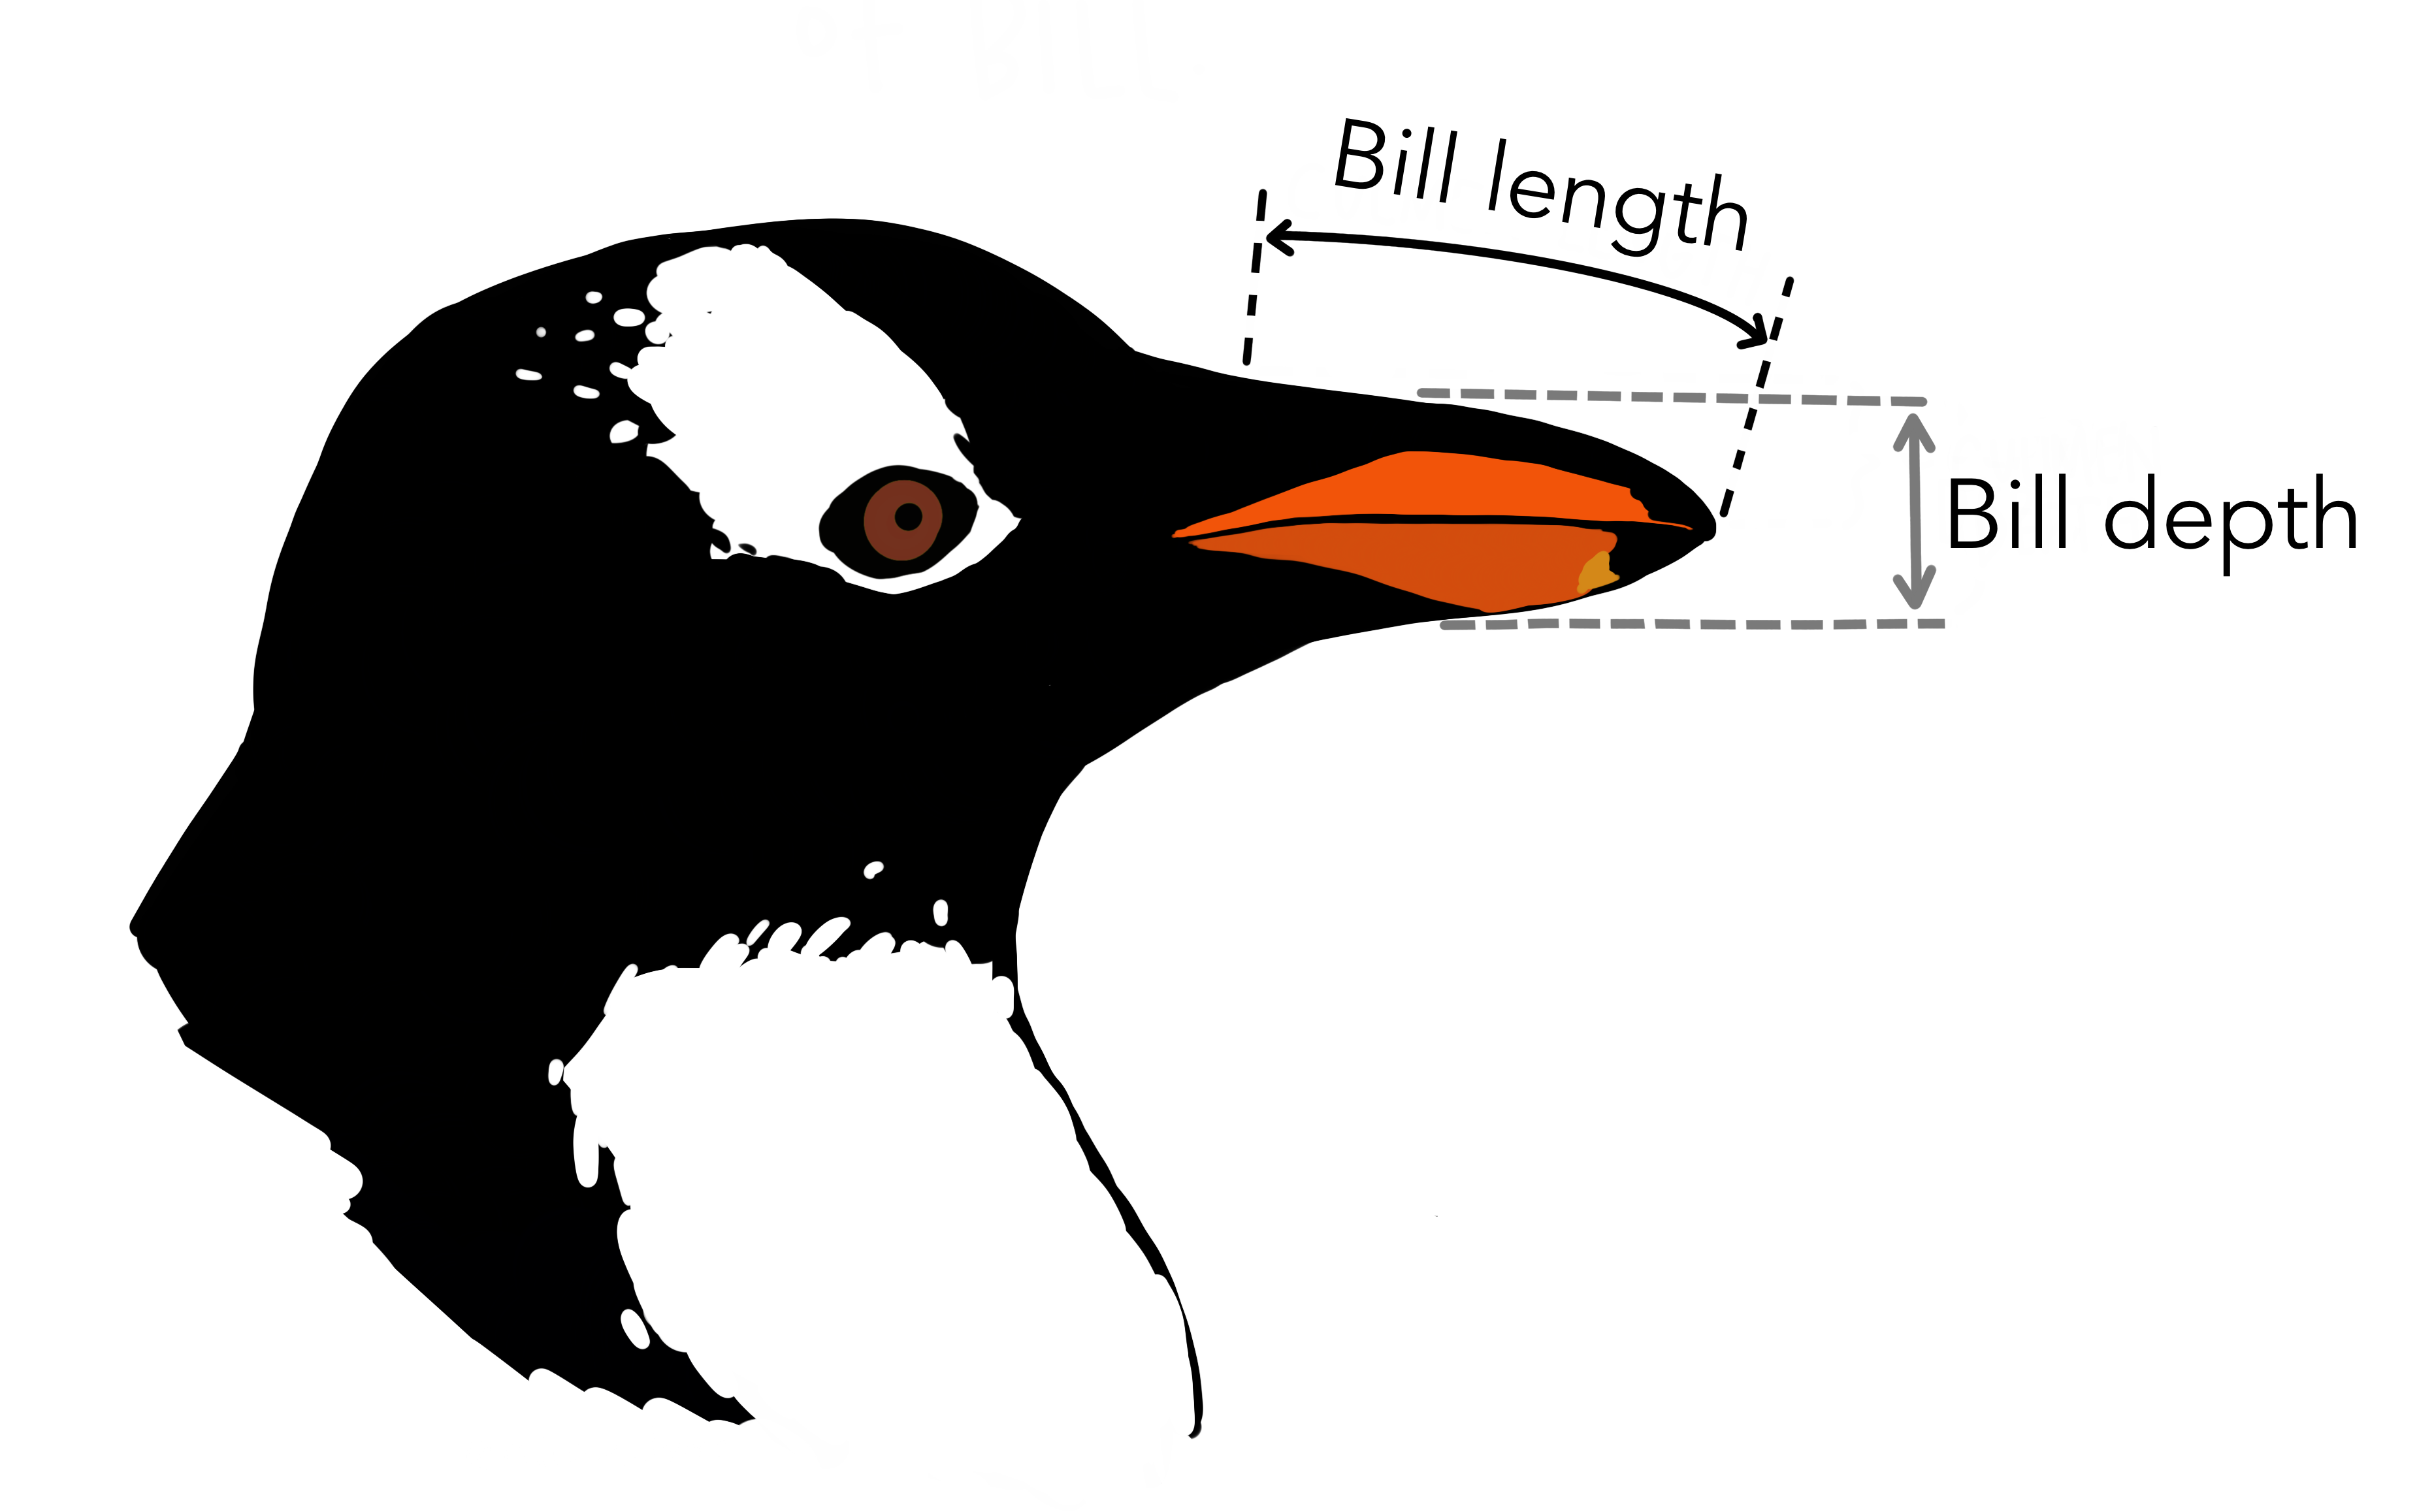
\includegraphics[width=2.08333in,height=1.5625in]{images/images_horst/palmer_penguin.png}

\end{col}

\end{cols}

Artwork by @allison\_horst

\end{tcolorbox}

\begin{tcolorbox}[enhanced jigsaw, breakable, colback=white, bottomrule=.15mm, leftrule=.75mm, colframe=quarto-callout-important-color-frame, arc=.35mm, rightrule=.15mm, toprule=.15mm, left=2mm, opacityback=0]

\begin{cols}

\begin{col}{0.90\textwidth}
How would you describe the scatterplot?

\end{col}

\begin{col}{0.10\textwidth}

\includegraphics[width=\textwidth,height=0.5in]{images/images_lecture/participate_icon.png}

\end{col}

\end{cols}

\begin{itemize}
\tightlist
\item
  Positive ``moderately linear''.
\item
  Teaching tip: draw an oval around the points. The thinner the oval the
  stronger the relationship. An approximate circle means no
  relationship.
\item
  Emphasize using the ``buzz words'' from the previous slide.
\item
  Some students may have noticed what appears to be three clusters! We
  will look at clusters in the next example.
\end{itemize}

\end{tcolorbox}

\begin{tcolorbox}[enhanced jigsaw, breakable, colback=white, bottomrule=.15mm, leftrule=.75mm, colframe=quarto-callout-note-color-frame, arc=.35mm, rightrule=.15mm, toprule=.15mm, left=2mm, opacityback=0]

\hypertarget{plot}{%
\subsubsection*{Plot}\label{plot}}
\addcontentsline{toc}{subsubsection}{Plot}

\begin{Shaded}
\begin{Highlighting}[]
\FunctionTok{ggplot}\NormalTok{(penguins, }\FunctionTok{aes}\NormalTok{(}\AttributeTok{x=}\NormalTok{flipper\_length\_mm, }\AttributeTok{y=}\NormalTok{bill\_length\_mm)) }\SpecialCharTok{+}
  \FunctionTok{geom\_point}\NormalTok{()}
\end{Highlighting}
\end{Shaded}

\begin{figure}[H]

{\centering 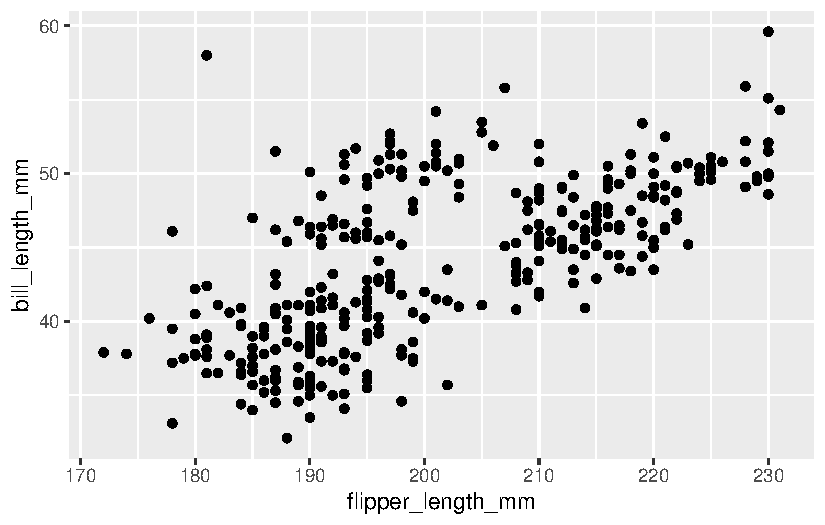
\includegraphics{03-content_files/figure-pdf/unnamed-chunk-4-1.pdf}

}

\caption{Fig A}

\end{figure}

\hypertarget{data}{%
\subsubsection*{Data}\label{data}}
\addcontentsline{toc}{subsubsection}{Data}

\begin{Shaded}
\begin{Highlighting}[]
\InformationTok{\textasciigrave{}\textasciigrave{}\textasciigrave{}\{r\}}

\FunctionTok{glimpse}\NormalTok{(penguins)}
\InformationTok{\textasciigrave{}\textasciigrave{}\textasciigrave{}}
\end{Highlighting}
\end{Shaded}

\begin{verbatim}
Rows: 344
Columns: 8
$ species           <fct> Adelie, Adelie, Adelie, Adelie, Adelie, Adelie, Adel~
$ island            <fct> Torgersen, Torgersen, Torgersen, Torgersen, Torgerse~
$ bill_length_mm    <dbl> 39.1, 39.5, 40.3, NA, 36.7, 39.3, 38.9, 39.2, 34.1, ~
$ bill_depth_mm     <dbl> 18.7, 17.4, 18.0, NA, 19.3, 20.6, 17.8, 19.6, 18.1, ~
$ flipper_length_mm <int> 181, 186, 195, NA, 193, 190, 181, 195, 193, 190, 186~
$ body_mass_g       <int> 3750, 3800, 3250, NA, 3450, 3650, 3625, 4675, 3475, ~
$ sex               <fct> male, female, female, NA, female, male, female, male~
$ year              <int> 2007, 2007, 2007, 2007, 2007, 2007, 2007, 2007, 2007~
\end{verbatim}

\end{tcolorbox}

\begin{tcolorbox}[enhanced jigsaw, breakable, colback=white, bottomrule=.15mm, leftrule=.75mm, colframe=quarto-callout-important-color-frame, arc=.35mm, rightrule=.15mm, toprule=.15mm, left=2mm, opacityback=0]

\begin{cols}

\begin{col}{0.90\textwidth}
How would you describe the scatterplot?

\end{col}

\begin{col}{0.10\textwidth}

\includegraphics[width=\textwidth,height=0.5in]{images/images_lecture/participate_icon.png}

\end{col}

\end{cols}

\begin{itemize}
\tightlist
\item
  Overall negative ``weakly linear''.
\item
  Teaching tip: draw an oval around the points.
\end{itemize}

\end{tcolorbox}

\begin{tcolorbox}[enhanced jigsaw, breakable, colback=white, bottomrule=.15mm, leftrule=.75mm, colframe=quarto-callout-important-color-frame, arc=.35mm, rightrule=.15mm, toprule=.15mm, left=2mm, opacityback=0]

But the clusters don't appear to be negative\ldots{} what variable might
be causing these two separate clusters?

\begin{itemize}
\tightlist
\item
  Since there are two your first instinct is probably the variable
  \texttt{sex}
\end{itemize}

\end{tcolorbox}

\begin{tcolorbox}[enhanced jigsaw, breakable, colback=white, bottomrule=.15mm, leftrule=.75mm, colframe=quarto-callout-note-color-frame, arc=.35mm, rightrule=.15mm, toprule=.15mm, left=2mm, opacityback=0]

\begin{Shaded}
\begin{Highlighting}[]
\InformationTok{\textasciigrave{}\textasciigrave{}\textasciigrave{}\{r\}}
\CommentTok{\#| eval: false}
\FunctionTok{ggplot}\NormalTok{(penguins, }\FunctionTok{aes}\NormalTok{(}\AttributeTok{x=}\NormalTok{flipper\_length\_mm, }\AttributeTok{y=}\NormalTok{bill\_depth\_mm)) }\SpecialCharTok{+}
  \FunctionTok{geom\_point}\NormalTok{()}
\InformationTok{\textasciigrave{}\textasciigrave{}\textasciigrave{}}
\end{Highlighting}
\end{Shaded}

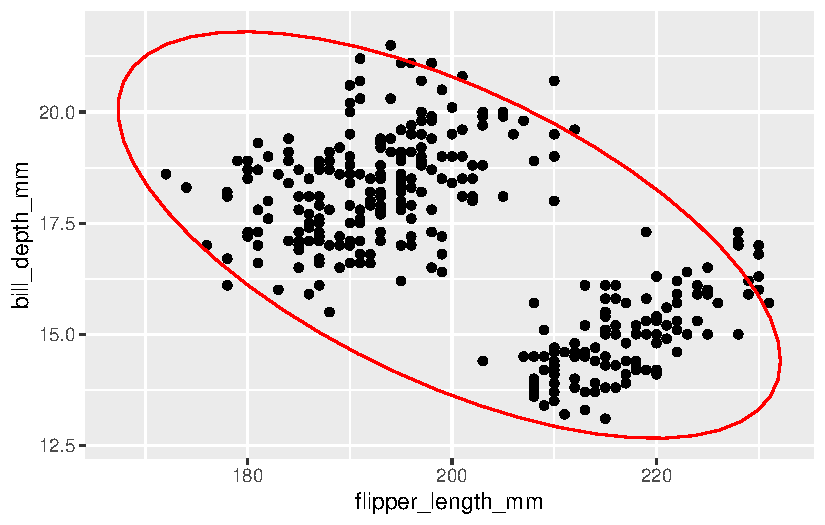
\includegraphics{03-content_files/figure-pdf/unnamed-chunk-7-1.pdf}

\end{tcolorbox}

\begin{tcolorbox}[enhanced jigsaw, breakable, colback=white, bottomrule=.15mm, leftrule=.75mm, colframe=quarto-callout-important-color-frame, arc=.35mm, rightrule=.15mm, toprule=.15mm, left=2mm, opacityback=0]
But \texttt{sex} is not the cause of the clusters. Try another
categorical variable that might cause different flipper and bill length.
\end{tcolorbox}

\begin{tcolorbox}[enhanced jigsaw, breakable, colback=white, bottomrule=.15mm, leftrule=.75mm, colframe=quarto-callout-note-color-frame, arc=.35mm, rightrule=.15mm, toprule=.15mm, left=2mm, opacityback=0]

\hypertarget{plot-1}{%
\subsubsection*{Plot}\label{plot-1}}
\addcontentsline{toc}{subsubsection}{Plot}

\begin{Shaded}
\begin{Highlighting}[]
\InformationTok{\textasciigrave{}\textasciigrave{}\textasciigrave{}\{r\}}
\CommentTok{\#| fig{-}cap: "Fig C"}
\FunctionTok{ggplot}\NormalTok{(penguins, }\FunctionTok{aes}\NormalTok{(}\AttributeTok{x=}\NormalTok{flipper\_length\_mm, }\AttributeTok{y=}\NormalTok{bill\_depth\_mm, }\AttributeTok{color =}\NormalTok{ sex)) }\SpecialCharTok{+}
  \FunctionTok{geom\_point}\NormalTok{()}
\InformationTok{\textasciigrave{}\textasciigrave{}\textasciigrave{}}
\end{Highlighting}
\end{Shaded}

\begin{figure}[H]

{\centering 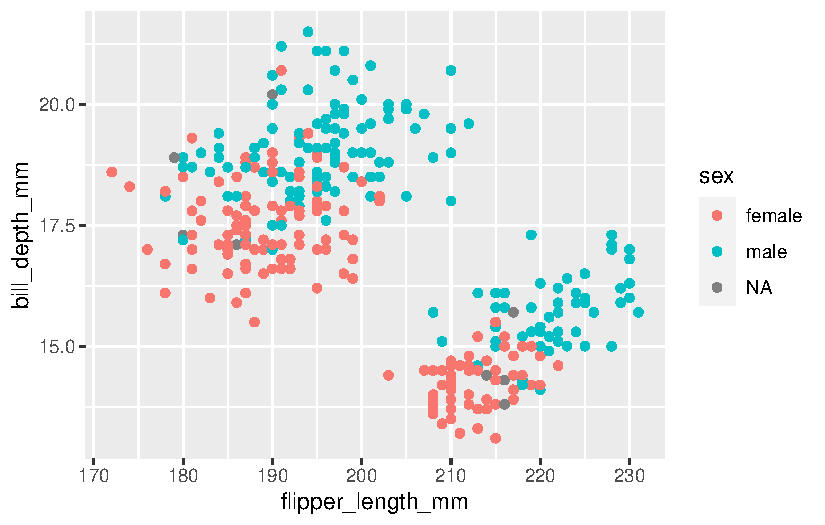
\includegraphics{03-content_files/figure-pdf/unnamed-chunk-8-1.pdf}

}

\caption{Fig C}

\end{figure}

\hypertarget{data-1}{%
\subsubsection*{Data}\label{data-1}}
\addcontentsline{toc}{subsubsection}{Data}

\begin{Shaded}
\begin{Highlighting}[]
\InformationTok{\textasciigrave{}\textasciigrave{}\textasciigrave{}\{r\}}

\FunctionTok{glimpse}\NormalTok{(penguins)}
\InformationTok{\textasciigrave{}\textasciigrave{}\textasciigrave{}}
\end{Highlighting}
\end{Shaded}

\begin{verbatim}
Rows: 344
Columns: 8
$ species           <fct> Adelie, Adelie, Adelie, Adelie, Adelie, Adelie, Adel~
$ island            <fct> Torgersen, Torgersen, Torgersen, Torgersen, Torgerse~
$ bill_length_mm    <dbl> 39.1, 39.5, 40.3, NA, 36.7, 39.3, 38.9, 39.2, 34.1, ~
$ bill_depth_mm     <dbl> 18.7, 17.4, 18.0, NA, 19.3, 20.6, 17.8, 19.6, 18.1, ~
$ flipper_length_mm <int> 181, 186, 195, NA, 193, 190, 181, 195, 193, 190, 186~
$ body_mass_g       <int> 3750, 3800, 3250, NA, 3450, 3650, 3625, 4675, 3475, ~
$ sex               <fct> male, female, female, NA, female, male, female, male~
$ year              <int> 2007, 2007, 2007, 2007, 2007, 2007, 2007, 2007, 2007~
\end{verbatim}

\end{tcolorbox}

\begin{tcolorbox}[enhanced jigsaw, breakable, colback=white, bottomrule=.15mm, leftrule=.75mm, colframe=quarto-callout-important-color-frame, arc=.35mm, rightrule=.15mm, toprule=.15mm, left=2mm, opacityback=0]
Now describe the scatterplot: Weakly positive linear for Adelie and
Chinstrap species. These two species appear to be similar with the
center of the grouping having a flipper length around 190 mm and bill
depth around 18.5mm. Gentoo also has a positive linear relationship,
perhaps more moderate than weak. Gentoo have a longer flipper but
shorter bill depth than the other 2 species.
\end{tcolorbox}

\begin{tcolorbox}[enhanced jigsaw, breakable, colback=white, bottomrule=.15mm, leftrule=.75mm, colframe=quarto-callout-note-color-frame, arc=.35mm, rightrule=.15mm, toprule=.15mm, left=2mm, opacityback=0]

\hypertarget{plot-2}{%
\subsubsection*{Plot}\label{plot-2}}
\addcontentsline{toc}{subsubsection}{Plot}

\begin{Shaded}
\begin{Highlighting}[]
\InformationTok{\textasciigrave{}\textasciigrave{}\textasciigrave{}\{r\}}
\CommentTok{\#| fig{-}cap: "Fig D"}
\FunctionTok{ggplot}\NormalTok{(penguins, }\FunctionTok{aes}\NormalTok{(}\AttributeTok{x=}\NormalTok{flipper\_length\_mm, }\AttributeTok{y=}\NormalTok{bill\_depth\_mm, }\AttributeTok{color =}\NormalTok{ species)) }\SpecialCharTok{+}
  \FunctionTok{geom\_point}\NormalTok{()}
\InformationTok{\textasciigrave{}\textasciigrave{}\textasciigrave{}}
\end{Highlighting}
\end{Shaded}

\begin{figure}[H]

{\centering 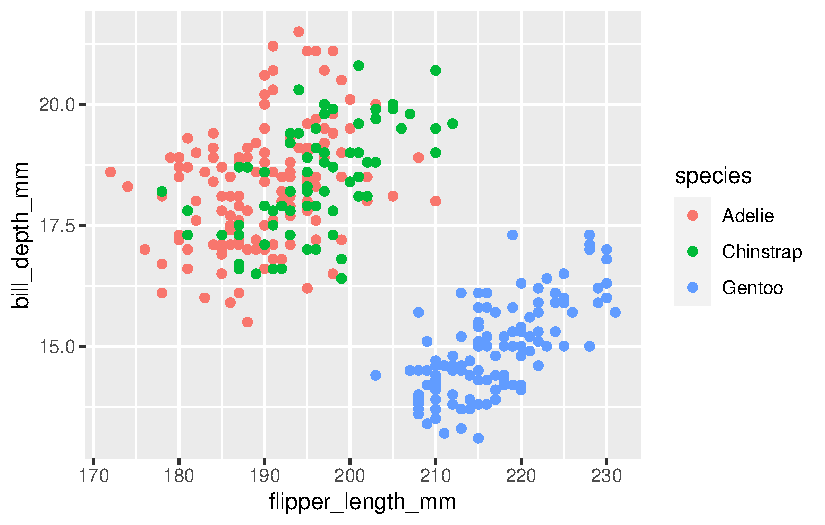
\includegraphics{03-content_files/figure-pdf/unnamed-chunk-10-1.pdf}

}

\caption{Fig D}

\end{figure}

\hypertarget{data-2}{%
\subsubsection*{Data}\label{data-2}}
\addcontentsline{toc}{subsubsection}{Data}

\begin{Shaded}
\begin{Highlighting}[]
\InformationTok{\textasciigrave{}\textasciigrave{}\textasciigrave{}\{r\}}

\FunctionTok{glimpse}\NormalTok{(penguins)}
\InformationTok{\textasciigrave{}\textasciigrave{}\textasciigrave{}}
\end{Highlighting}
\end{Shaded}

\begin{verbatim}
Rows: 344
Columns: 8
$ species           <fct> Adelie, Adelie, Adelie, Adelie, Adelie, Adelie, Adel~
$ island            <fct> Torgersen, Torgersen, Torgersen, Torgersen, Torgerse~
$ bill_length_mm    <dbl> 39.1, 39.5, 40.3, NA, 36.7, 39.3, 38.9, 39.2, 34.1, ~
$ bill_depth_mm     <dbl> 18.7, 17.4, 18.0, NA, 19.3, 20.6, 17.8, 19.6, 18.1, ~
$ flipper_length_mm <int> 181, 186, 195, NA, 193, 190, 181, 195, 193, 190, 186~
$ body_mass_g       <int> 3750, 3800, 3250, NA, 3450, 3650, 3625, 4675, 3475, ~
$ sex               <fct> male, female, female, NA, female, male, female, male~
$ year              <int> 2007, 2007, 2007, 2007, 2007, 2007, 2007, 2007, 2007~
\end{verbatim}

\end{tcolorbox}

\begin{tcolorbox}[enhanced jigsaw, breakable, colback=white, bottomrule=.15mm, leftrule=.75mm, colframe=quarto-callout-note-color-frame, arc=.35mm, rightrule=.15mm, toprule=.15mm, left=2mm, opacityback=0]

\begin{enumerate}
\def\labelenumi{\arabic{enumi}.}
\tightlist
\item
\end{enumerate}

\begin{Shaded}
\begin{Highlighting}[]
\InformationTok{\textasciigrave{}\textasciigrave{}\textasciigrave{}\{r\}}
\CommentTok{\#| eval: false}
\FunctionTok{ggplot}\NormalTok{(penguins, }\FunctionTok{aes}\NormalTok{(}\AttributeTok{x=}\NormalTok{flipper\_length\_mm, }\AttributeTok{y=}\NormalTok{bill\_depth\_mm)) }\SpecialCharTok{+}
  \FunctionTok{geom\_point}\NormalTok{() }\SpecialCharTok{+}
\InformationTok{\textasciigrave{}\textasciigrave{}\textasciigrave{}}
\end{Highlighting}
\end{Shaded}

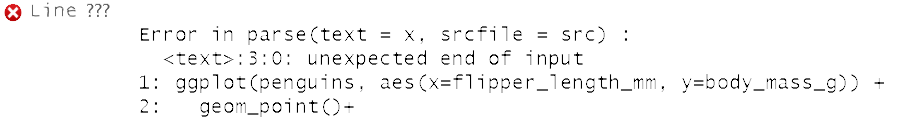
\includegraphics[width=4.16667in,height=0.78125in]{images/images_lecture/error_2a.png}

Plus sign to nowhere. What would happen if you type ``1+2+'' into a
calculator? An error!

\begin{enumerate}
\def\labelenumi{\arabic{enumi}.}
\setcounter{enumi}{1}
\tightlist
\item
\end{enumerate}

\begin{Shaded}
\begin{Highlighting}[]
\InformationTok{\textasciigrave{}\textasciigrave{}\textasciigrave{}\{r\}}
\CommentTok{\#| eval: false}
\FunctionTok{ggplot}\NormalTok{(penguins, }\FunctionTok{aes}\NormalTok{(}\AttributeTok{x=}\NormalTok{flipper\_length\_mm, }\AttributeTok{y=}\NormalTok{bill\_depth\_mm) }\SpecialCharTok{+}
  \FunctionTok{geom\_point}\NormalTok{()}
\StringTok{\textasciigrave{}\textasciigrave{}\textasciigrave{}}
\end{Highlighting}
\end{Shaded}

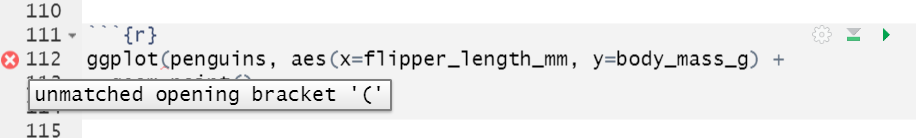
\includegraphics[width=4.16667in,height=0.78125in]{images/images_lecture/error_2b.png}

All parenthesis must me closed!

\begin{enumerate}
\def\labelenumi{\arabic{enumi}.}
\setcounter{enumi}{2}
\tightlist
\item
\end{enumerate}

\begin{Shaded}
\begin{Highlighting}[]
\InformationTok{\textasciigrave{}\textasciigrave{}\textasciigrave{}\{r\}}
\CommentTok{\#| eval: false}
\FunctionTok{ggplot}\NormalTok{(Penguins, }\FunctionTok{aes}\NormalTok{(}\AttributeTok{x=}\NormalTok{Flipper\_length\_mm, }\AttributeTok{y=}\NormalTok{Bill\_depth\_mm) }\SpecialCharTok{+}
  \FunctionTok{geom\_point}\NormalTok{()}
\StringTok{\textasciigrave{}\textasciigrave{}\textasciigrave{}}
\end{Highlighting}
\end{Shaded}


\includegraphics[width=4.16667in,height=0.78125in]{images/images_lecture/error_2c.png}

R is case sensitive! Make sure the data and variable names match
EXACTLY.

\end{tcolorbox}

\begin{tcolorbox}[enhanced jigsaw, breakable, colback=white, bottomrule=.15mm, leftrule=.75mm, colframe=quarto-callout-note-color-frame, arc=.35mm, rightrule=.15mm, toprule=.15mm, left=2mm, opacityback=0]

\begin{itemize}
\item
  \href{https://www.rstudio.com/resources/cheatsheets/}{ggplot2
  cheatsheet link}
\item
  Numerical vs Categorical data examples:
\end{itemize}

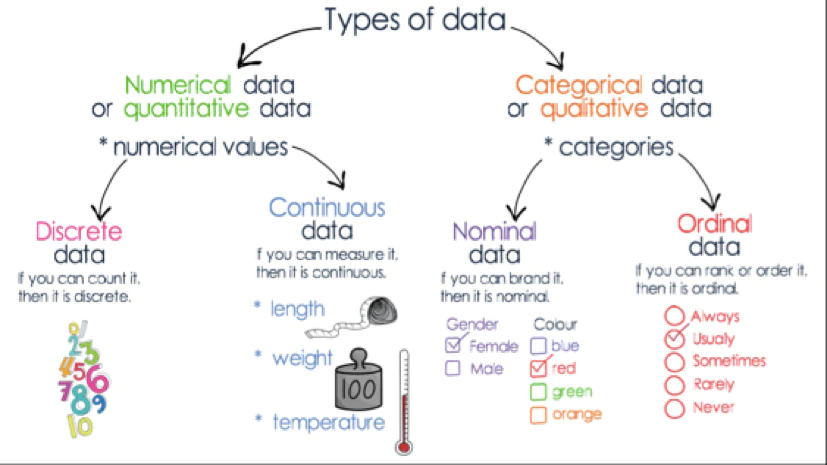
\includegraphics[width=\textwidth,height=2.5in]{images/images_lecture/data_types.png}
\end{tcolorbox}

\hypertarget{activity-solution-1}{%
\section*{Activity Solution}\label{activity-solution-1}}
\addcontentsline{toc}{section}{Activity Solution}

Need to add. See RStudio Cloud TA Solutions for now.

\hypertarget{homework-2}{%
\section*{Homework}\label{homework-2}}
\addcontentsline{toc}{section}{Homework}

\begin{itemize}
\item
  Complete and submit Activity 02
\item
  Read Sections 2.4 - 2.6 of the book
\item
  Complete and submit Reading Check 03\_ggplot2
\end{itemize}

\bookmarksetup{startatroot}

\hypertarget{day-04}{%
\chapter*{Day 04}\label{day-04}}
\addcontentsline{toc}{chapter}{Day 04}

Today's lesson covers
\href{https://nustat.github.io/intro-stat-data-sci/02-visualization.html}{Section
2.4 - 2.6} and focuses on making linegraphs and histograms with
\texttt{ggplot()}.

\begin{tcolorbox}[enhanced jigsaw, toptitle=1mm, colback=white, arc=.35mm, rightrule=.15mm, titlerule=0mm, left=2mm, breakable, bottomtitle=1mm, bottomrule=.15mm, leftrule=.75mm, title={Agenda}, colframe=quarto-callout-note-color-frame, opacitybacktitle=0.6, toprule=.15mm, colbacktitle=quarto-callout-note-color!10!white, coltitle=black, opacityback=0]
\textasciitilde{} 15 min Slide deck

\textasciitilde{} 25 min Students work on Activity 02

\textasciitilde{} 10 min Work through a select problem in detail from
the activity as a class
\end{tcolorbox}

\hypertarget{slide-deck-3}{%
\section*{Slide Deck}\label{slide-deck-3}}
\addcontentsline{toc}{section}{Slide Deck}

\begin{tcolorbox}[enhanced jigsaw, breakable, colback=white, bottomrule=.15mm, leftrule=.75mm, colframe=quarto-callout-note-color-frame, arc=.35mm, rightrule=.15mm, toprule=.15mm, left=2mm, opacityback=0]

\begin{enumerate}
\def\labelenumi{\arabic{enumi}.}
\tightlist
\item
  Create a linegraph
\item
  Create a histogram
\item
  Properly describe a linegraph and histogram
\item
  Facet graphs based on subgroups
\end{enumerate}

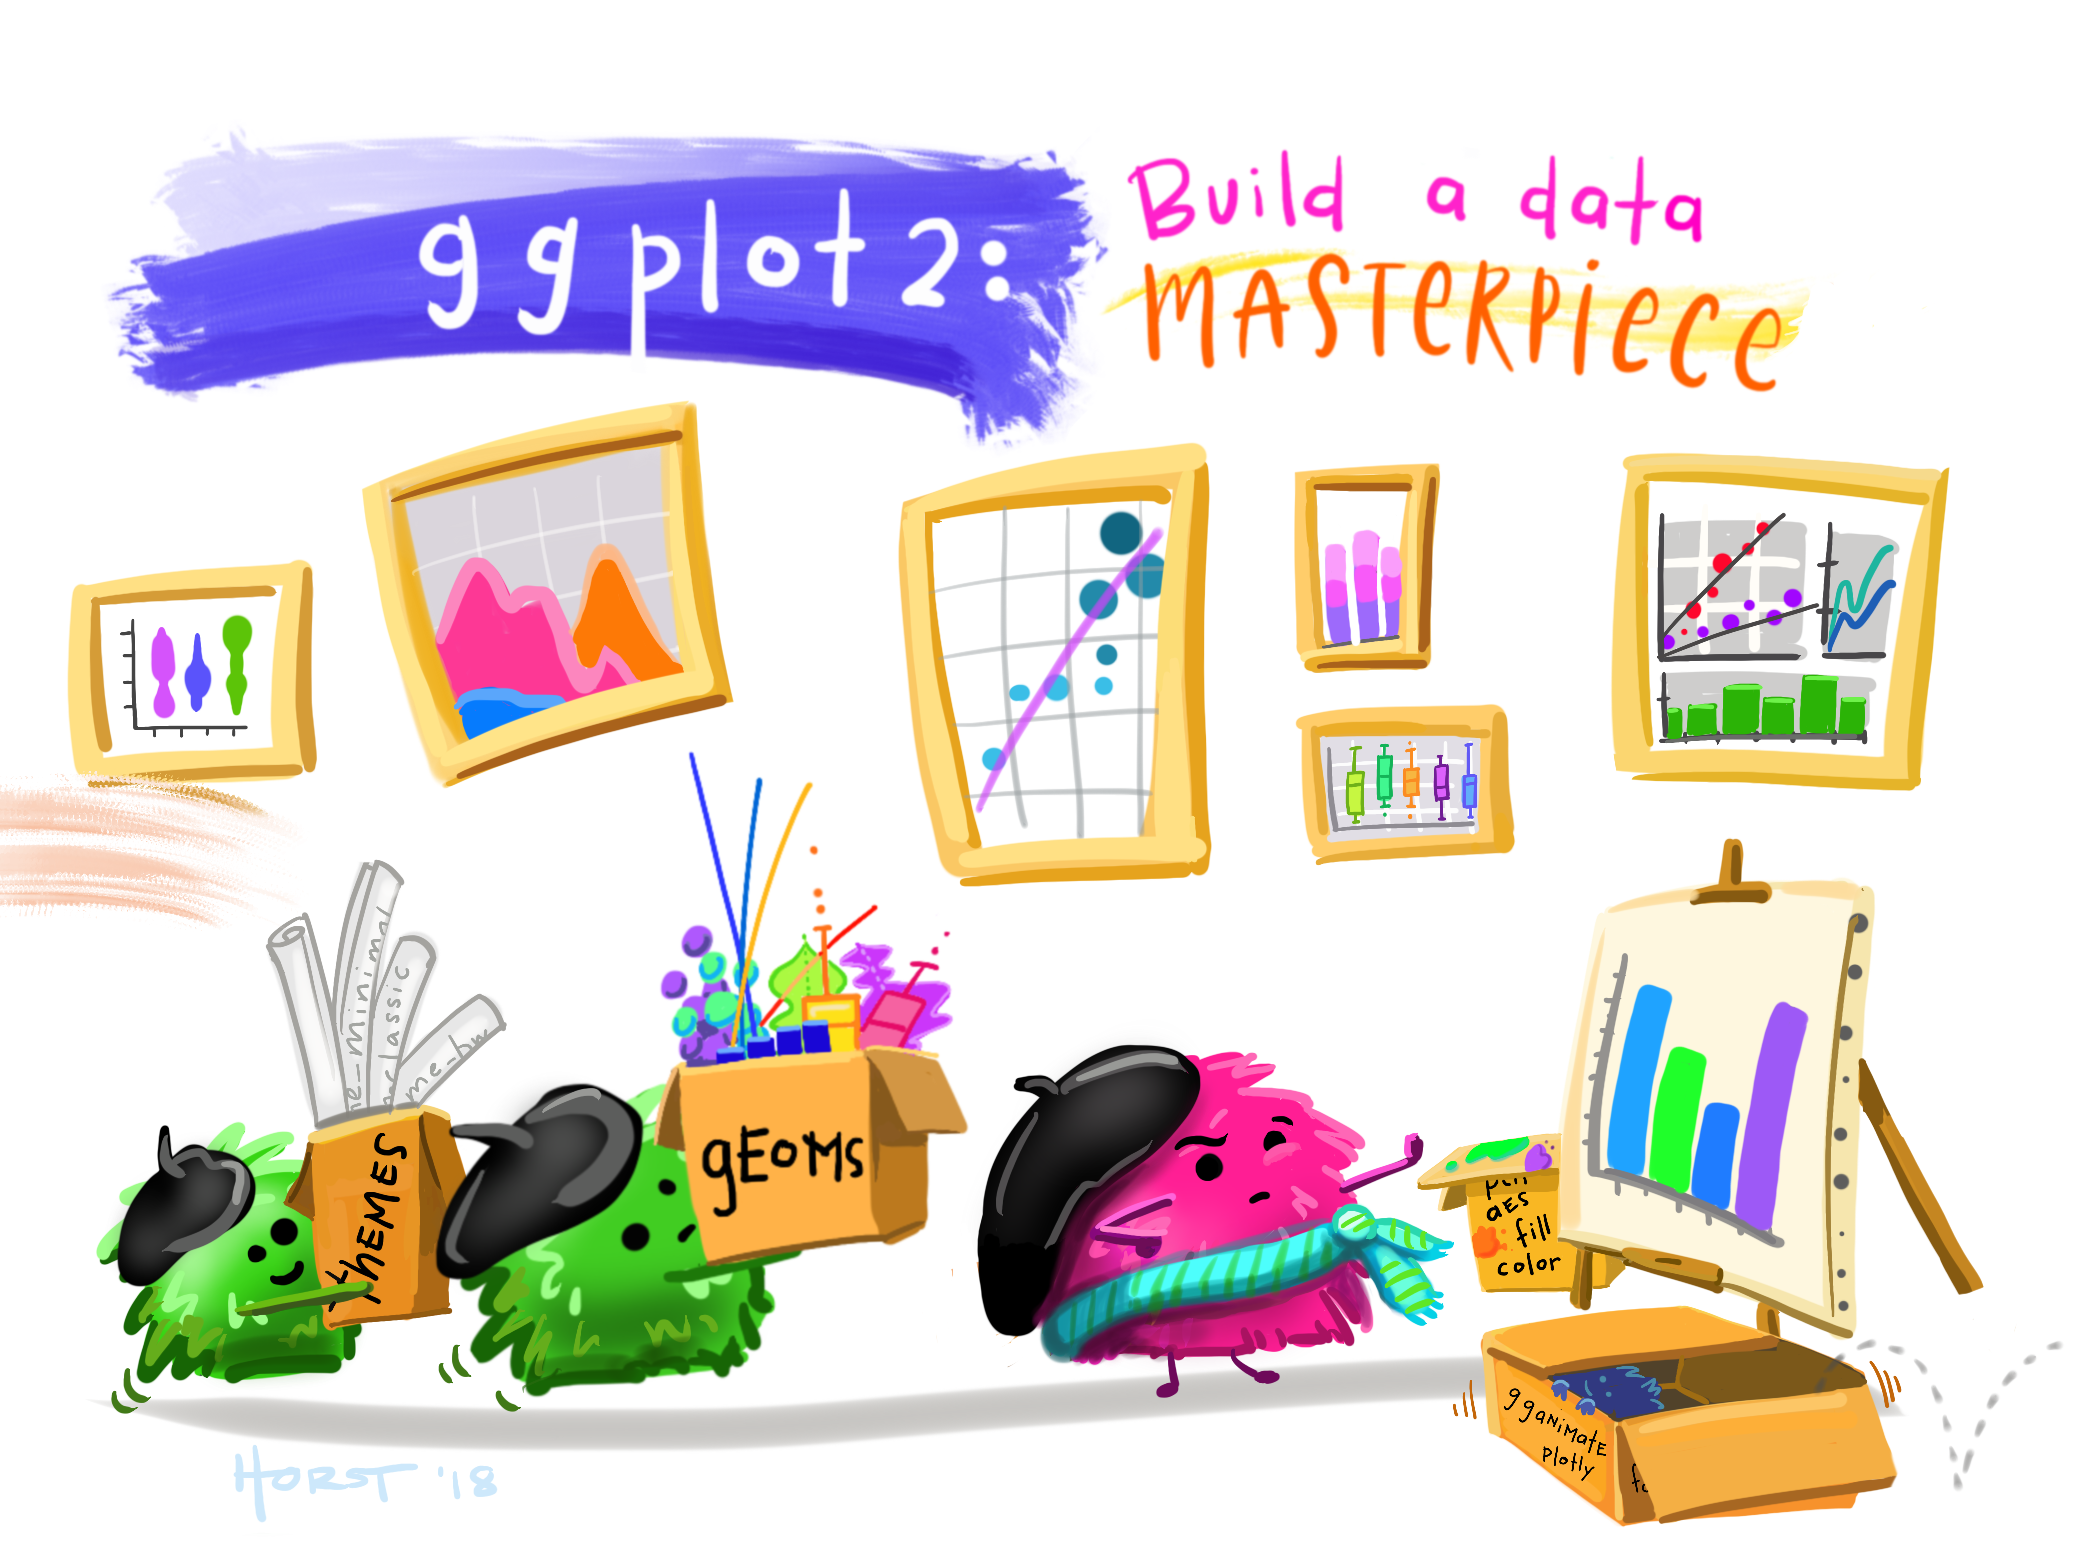
\includegraphics[width=\textwidth,height=1in]{images/images_horst/ggplot2_masterpiece.png}
Artwork by @allison\_horst

\end{tcolorbox}

\begin{tcolorbox}[enhanced jigsaw, breakable, colback=white, bottomrule=.15mm, leftrule=.75mm, colframe=quarto-callout-note-color-frame, arc=.35mm, rightrule=.15mm, toprule=.15mm, left=2mm, opacityback=0]

Linegraphs show the \textbf{relationship} between 2 \textbf{numerical}
variables.

The explanatory (x-axis) variable \textbf{must be of} sequential
ordering.

\textbf{Linegraph syntax in R:}

\begin{Shaded}
\begin{Highlighting}[]
\FunctionTok{ggplot}\NormalTok{(}\AttributeTok{data=}\NormalTok{ my\_data, }\AttributeTok{mapping =} \FunctionTok{aes}\NormalTok{(}\AttributeTok{x =}\NormalTok{ var1, }\AttributeTok{y =}\NormalTok{ var2)) }\SpecialCharTok{+}
  \FunctionTok{geom\_line}\NormalTok{()}
\end{Highlighting}
\end{Shaded}

\end{tcolorbox}

\begin{tcolorbox}[enhanced jigsaw, breakable, colback=white, bottomrule=.15mm, leftrule=.75mm, colframe=quarto-callout-note-color-frame, arc=.35mm, rightrule=.15mm, toprule=.15mm, left=2mm, opacityback=0]

When describing linegraphs\ldots{}

\begin{itemize}
\tightlist
\item
  Look for pattern going from left to right.
\item
  Classify association as positive, negative, or no association.
\item
  Classify relationship as linear or non linear.
\item
  Check x and y scales to make sure they are appropriate.
\end{itemize}

\end{tcolorbox}

\begin{tcolorbox}[enhanced jigsaw, breakable, colback=white, bottomrule=.15mm, leftrule=.75mm, colframe=quarto-callout-note-color-frame, arc=.35mm, rightrule=.15mm, toprule=.15mm, left=2mm, opacityback=0]

\begin{itemize}
\item
  Histograms are used to visualize the \textbf{distribution} of a single
  \textbf{numerical} variable.
\item
  Histograms display \textbf{numerical} data by grouping data into bins
  of equal width.
\item
  There is \textbf{no} `y' position aesthetic for
  \texttt{geom\_histogram()} because we are investigating a single
  variable.
\end{itemize}

\end{tcolorbox}

\begin{tcolorbox}[enhanced jigsaw, breakable, colback=white, bottomrule=.15mm, leftrule=.75mm, colframe=quarto-callout-note-color-frame, arc=.35mm, rightrule=.15mm, toprule=.15mm, left=2mm, opacityback=0]

\textbf{Histogram syntax in R:}

\begin{Shaded}
\begin{Highlighting}[]
\FunctionTok{ggplot}\NormalTok{(}\AttributeTok{data=}\NormalTok{ my\_data, }\FunctionTok{aes}\NormalTok{(}\AttributeTok{x =}\NormalTok{ var1)) }\SpecialCharTok{+}
  \FunctionTok{geom\_histogram}\NormalTok{(}\AttributeTok{color =} \StringTok{"white"}\NormalTok{, }\AttributeTok{fill =} \StringTok{"blue"}\NormalTok{, }\AttributeTok{bins =} \DecValTok{10}\NormalTok{)}
\end{Highlighting}
\end{Shaded}

There are 3 things we look and describe when inspecting a histogram:

\begin{itemize}
\tightlist
\item
  shape (skew and modality)
\item
  center (mean or median)
\item
  spread (range, IQR, or standard deviation)
\end{itemize}

Not all distributions have a simple recognizable shape!

Type \texttt{colors()} in the \textbf{console} to view all possible
colors.

\end{tcolorbox}

\begin{tcolorbox}[enhanced jigsaw, breakable, colback=white, bottomrule=.15mm, leftrule=.75mm, colframe=quarto-callout-note-color-frame, arc=.35mm, rightrule=.15mm, toprule=.15mm, left=2mm, opacityback=0]

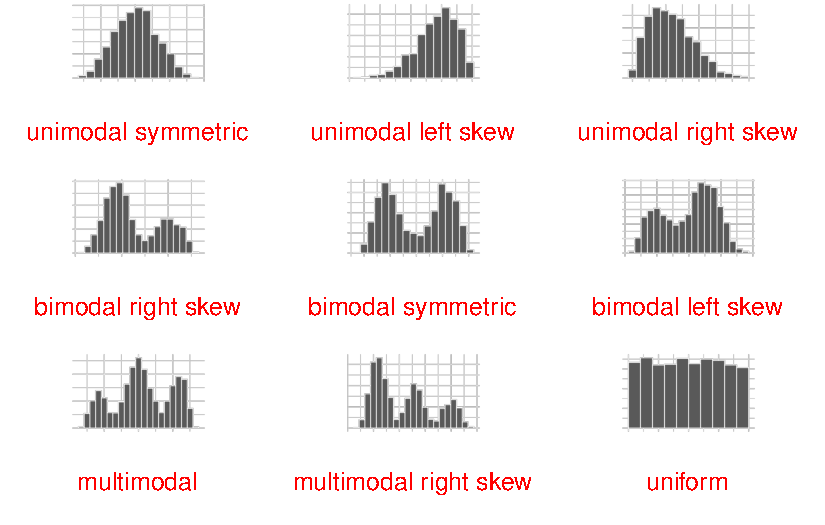
\includegraphics{04-content_files/figure-pdf/unnamed-chunk-2-1.pdf}

\end{tcolorbox}

\begin{tcolorbox}[enhanced jigsaw, breakable, colback=white, bottomrule=.15mm, leftrule=.75mm, colframe=quarto-callout-important-color-frame, arc=.35mm, rightrule=.15mm, toprule=.15mm, left=2mm, opacityback=0]

Teaching tip: open up the shiny app so student's can see how the bins
change as you move the slider.

Which bin is best?

\begin{itemize}
\tightlist
\item
  18 bins
\item
  emphasize that there is a broad range of bin sizes that would work
  well. You want to make sure you can see the shape but not every little
  up and down.
\end{itemize}

Describe the districution? - center around 3750 - spread in terms of
range is \textasciitilde2500 to 6500 - right skewed and ``fairly''
unimodal (could argue there is a small peak around 4750 and 5250)


\includegraphics[width=\textwidth,height=0.5in]{images/images_lecture/participate_icon.png}

\end{tcolorbox}

\begin{tcolorbox}[enhanced jigsaw, breakable, colback=white, bottomrule=.15mm, leftrule=.75mm, colframe=quarto-callout-note-color-frame, arc=.35mm, rightrule=.15mm, toprule=.15mm, left=2mm, opacityback=0]

Which bin size is most appropriate and describe the distribution of
penguin body mass.

\hypertarget{bins-7}{%
\subsubsection*{Bins = 7}\label{bins-7}}
\addcontentsline{toc}{subsubsection}{Bins = 7}

\begin{Shaded}
\begin{Highlighting}[]
\InformationTok{\textasciigrave{}\textasciigrave{}\textasciigrave{}\{r\}}

\FunctionTok{ggplot}\NormalTok{(penguins, }\FunctionTok{aes}\NormalTok{(}\AttributeTok{x=}\NormalTok{penguins}\SpecialCharTok{$}\NormalTok{body\_mass\_g)) }\SpecialCharTok{+}
    \FunctionTok{geom\_histogram}\NormalTok{(}\AttributeTok{color =} \StringTok{"white"}\NormalTok{, }
                   \AttributeTok{fill =} \StringTok{"lightblue"}\NormalTok{, }
                   \AttributeTok{bins =} \DecValTok{7}\NormalTok{)}\SpecialCharTok{+}
    \FunctionTok{labs}\NormalTok{(}\AttributeTok{title =} \StringTok{"Palmer Penguins Distribution of Body Mass"}\NormalTok{,}
           \AttributeTok{x =} \StringTok{"Body Mass (g)"}\NormalTok{)}
\InformationTok{\textasciigrave{}\textasciigrave{}\textasciigrave{}}
\end{Highlighting}
\end{Shaded}

\begin{figure}[H]

{\centering 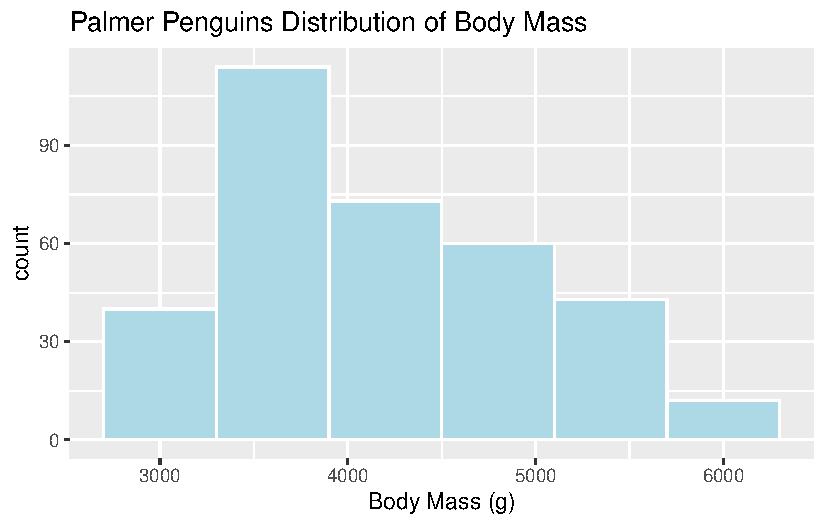
\includegraphics{04-content_files/figure-pdf/unnamed-chunk-3-1.pdf}

}

\end{figure}

\hypertarget{bins-18}{%
\subsubsection*{Bins = 18}\label{bins-18}}
\addcontentsline{toc}{subsubsection}{Bins = 18}

\begin{Shaded}
\begin{Highlighting}[]
\InformationTok{\textasciigrave{}\textasciigrave{}\textasciigrave{}\{r\}}

\FunctionTok{ggplot}\NormalTok{(penguins, }\FunctionTok{aes}\NormalTok{(}\AttributeTok{x=}\NormalTok{penguins}\SpecialCharTok{$}\NormalTok{body\_mass\_g)) }\SpecialCharTok{+}
    \FunctionTok{geom\_histogram}\NormalTok{(}\AttributeTok{color =} \StringTok{"white"}\NormalTok{, }
                   \AttributeTok{fill =} \StringTok{"lightblue"}\NormalTok{, }
                   \AttributeTok{bins =} \DecValTok{18}\NormalTok{)}\SpecialCharTok{+}
    \FunctionTok{labs}\NormalTok{(}\AttributeTok{title =} \StringTok{"Palmer Penguins Distribution of Body Mass"}\NormalTok{,}
           \AttributeTok{x =} \StringTok{"Body Mass (g)"}\NormalTok{)}
\InformationTok{\textasciigrave{}\textasciigrave{}\textasciigrave{}}
\end{Highlighting}
\end{Shaded}

\begin{figure}[H]

{\centering 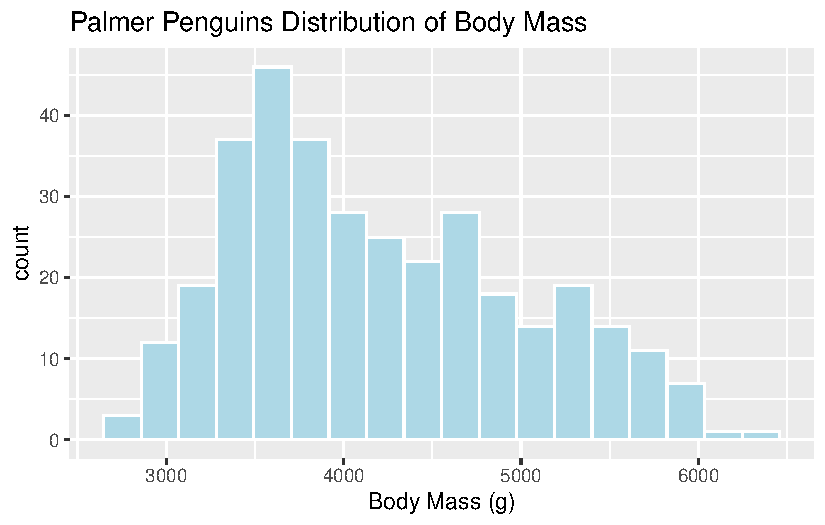
\includegraphics{04-content_files/figure-pdf/unnamed-chunk-4-1.pdf}

}

\end{figure}

\hypertarget{bins-29}{%
\subsubsection*{Bins = 29}\label{bins-29}}
\addcontentsline{toc}{subsubsection}{Bins = 29}

\begin{Shaded}
\begin{Highlighting}[]
\InformationTok{\textasciigrave{}\textasciigrave{}\textasciigrave{}\{r\}}

\FunctionTok{ggplot}\NormalTok{(penguins, }\FunctionTok{aes}\NormalTok{(}\AttributeTok{x=}\NormalTok{penguins}\SpecialCharTok{$}\NormalTok{body\_mass\_g)) }\SpecialCharTok{+}
    \FunctionTok{geom\_histogram}\NormalTok{(}\AttributeTok{color =} \StringTok{"white"}\NormalTok{, }
                   \AttributeTok{fill =} \StringTok{"lightblue"}\NormalTok{, }
                   \AttributeTok{bins =} \DecValTok{29}\NormalTok{)}\SpecialCharTok{+}
    \FunctionTok{labs}\NormalTok{(}\AttributeTok{title =} \StringTok{"Palmer Penguins Distribution of Body Mass"}\NormalTok{,}
           \AttributeTok{x =} \StringTok{"Body Mass (g)"}\NormalTok{)}
\InformationTok{\textasciigrave{}\textasciigrave{}\textasciigrave{}}
\end{Highlighting}
\end{Shaded}

\begin{figure}[H]

{\centering 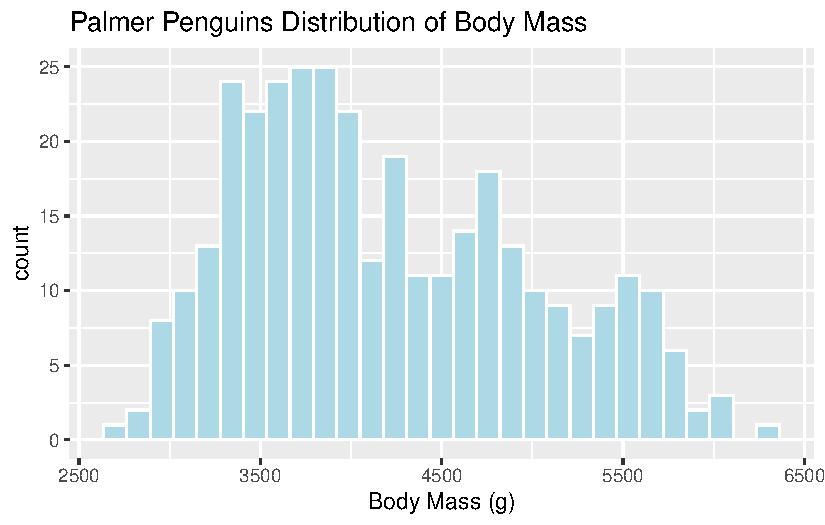
\includegraphics{04-content_files/figure-pdf/unnamed-chunk-5-1.pdf}

}

\end{figure}

https://northwestern-university.shinyapps.io/lec03\_histogram/

\end{tcolorbox}

\begin{tcolorbox}[enhanced jigsaw, breakable, colback=white, bottomrule=.15mm, leftrule=.75mm, colframe=quarto-callout-important-color-frame, arc=.35mm, rightrule=.15mm, toprule=.15mm, left=2mm, opacityback=0]

Teaching tip: open up the shiny app so student's can see how the bins
change as you move the slider.

Which bin is best?

\begin{itemize}
\tightlist
\item
  15 bins
\end{itemize}

Describe the districution.

\begin{itemize}
\tightlist
\item
  bimodal and right skewed
\item
  center of peaks around 190 and 215
\item
  spread in terms of range is \textasciitilde170 to 230
\end{itemize}


\includegraphics[width=\textwidth,height=0.5in]{images/images_lecture/participate_icon.png}

\end{tcolorbox}

\begin{tcolorbox}[enhanced jigsaw, breakable, colback=white, bottomrule=.15mm, leftrule=.75mm, colframe=quarto-callout-note-color-frame, arc=.35mm, rightrule=.15mm, toprule=.15mm, left=2mm, opacityback=0]

Which bin size is most appropriate and describe the distribution of
penguin flipper length.

\hypertarget{bins-15}{%
\subsubsection*{Bins = 15}\label{bins-15}}
\addcontentsline{toc}{subsubsection}{Bins = 15}

\begin{Shaded}
\begin{Highlighting}[]
\InformationTok{\textasciigrave{}\textasciigrave{}\textasciigrave{}\{r\}}

  \FunctionTok{ggplot}\NormalTok{(penguins, }\FunctionTok{aes}\NormalTok{(}\AttributeTok{x=}\NormalTok{penguins}\SpecialCharTok{$}\NormalTok{flipper\_length\_mm )) }\SpecialCharTok{+}
    \FunctionTok{geom\_histogram}\NormalTok{(}\AttributeTok{color =} \StringTok{"white"}\NormalTok{, }
                   \AttributeTok{fill =} \StringTok{"tomato1"}\NormalTok{, }
                   \AttributeTok{bins =} \DecValTok{15}\NormalTok{)}\SpecialCharTok{+}
    \FunctionTok{labs}\NormalTok{(}\AttributeTok{title =} \StringTok{"Palmer Penguins Distribution of Flipper Length"}\NormalTok{,}
           \AttributeTok{x =} \StringTok{"Flipper Length (mm)"}\NormalTok{)}
\InformationTok{\textasciigrave{}\textasciigrave{}\textasciigrave{}}
\end{Highlighting}
\end{Shaded}

\begin{figure}[H]

{\centering 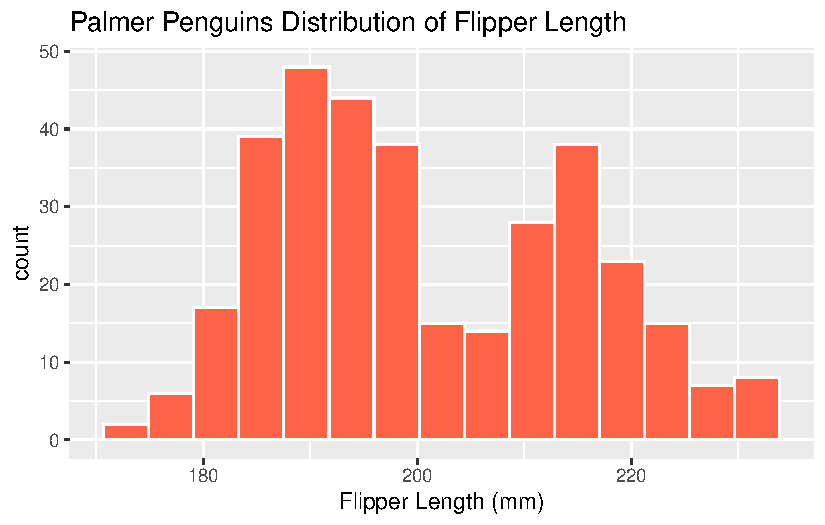
\includegraphics{04-content_files/figure-pdf/unnamed-chunk-6-1.pdf}

}

\end{figure}

\hypertarget{bins-25}{%
\subsubsection*{Bins = 25}\label{bins-25}}
\addcontentsline{toc}{subsubsection}{Bins = 25}

\begin{Shaded}
\begin{Highlighting}[]
\InformationTok{\textasciigrave{}\textasciigrave{}\textasciigrave{}\{r\}}

  \FunctionTok{ggplot}\NormalTok{(penguins, }\FunctionTok{aes}\NormalTok{(}\AttributeTok{x=}\NormalTok{penguins}\SpecialCharTok{$}\NormalTok{flipper\_length\_mm )) }\SpecialCharTok{+}
    \FunctionTok{geom\_histogram}\NormalTok{(}\AttributeTok{color =} \StringTok{"white"}\NormalTok{, }
                   \AttributeTok{fill =} \StringTok{"tomato1"}\NormalTok{, }
                   \AttributeTok{bins =} \DecValTok{25}\NormalTok{)}\SpecialCharTok{+}
    \FunctionTok{labs}\NormalTok{(}\AttributeTok{title =} \StringTok{"Palmer Penguins Distribution of Flipper Length"}\NormalTok{,}
           \AttributeTok{x =} \StringTok{"Flipper Length (mm)"}\NormalTok{)}
\InformationTok{\textasciigrave{}\textasciigrave{}\textasciigrave{}}
\end{Highlighting}
\end{Shaded}

\begin{figure}[H]

{\centering 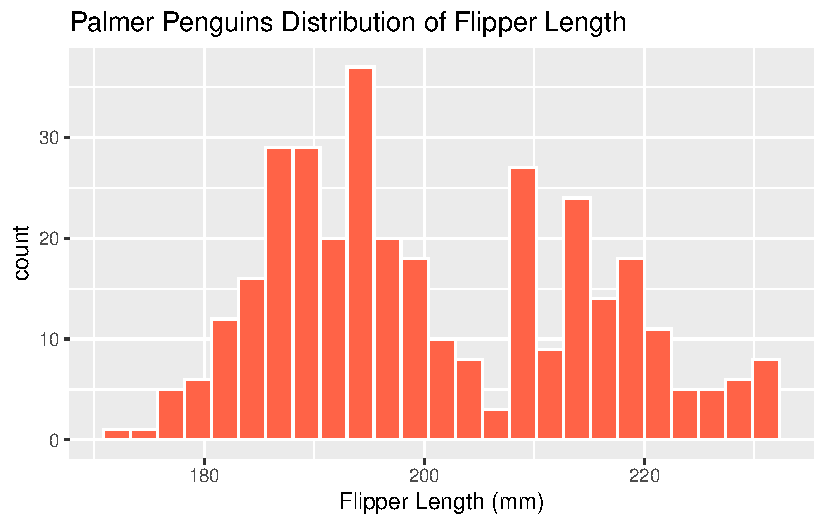
\includegraphics{04-content_files/figure-pdf/unnamed-chunk-7-1.pdf}

}

\end{figure}

\hypertarget{bins-35}{%
\subsubsection*{Bins = 35}\label{bins-35}}
\addcontentsline{toc}{subsubsection}{Bins = 35}

\begin{Shaded}
\begin{Highlighting}[]
\InformationTok{\textasciigrave{}\textasciigrave{}\textasciigrave{}\{r\}}

  \FunctionTok{ggplot}\NormalTok{(penguins, }\FunctionTok{aes}\NormalTok{(}\AttributeTok{x=}\NormalTok{penguins}\SpecialCharTok{$}\NormalTok{flipper\_length\_mm )) }\SpecialCharTok{+}
    \FunctionTok{geom\_histogram}\NormalTok{(}\AttributeTok{color =} \StringTok{"white"}\NormalTok{, }
                   \AttributeTok{fill =} \StringTok{"tomato1"}\NormalTok{, }
                   \AttributeTok{bins =} \DecValTok{35}\NormalTok{)}\SpecialCharTok{+}
    \FunctionTok{labs}\NormalTok{(}\AttributeTok{title =} \StringTok{"Palmer Penguins Distribution of Flipper Length"}\NormalTok{,}
           \AttributeTok{x =} \StringTok{"Flipper Length (mm)"}\NormalTok{)}
\InformationTok{\textasciigrave{}\textasciigrave{}\textasciigrave{}}
\end{Highlighting}
\end{Shaded}

\begin{figure}[H]

{\centering 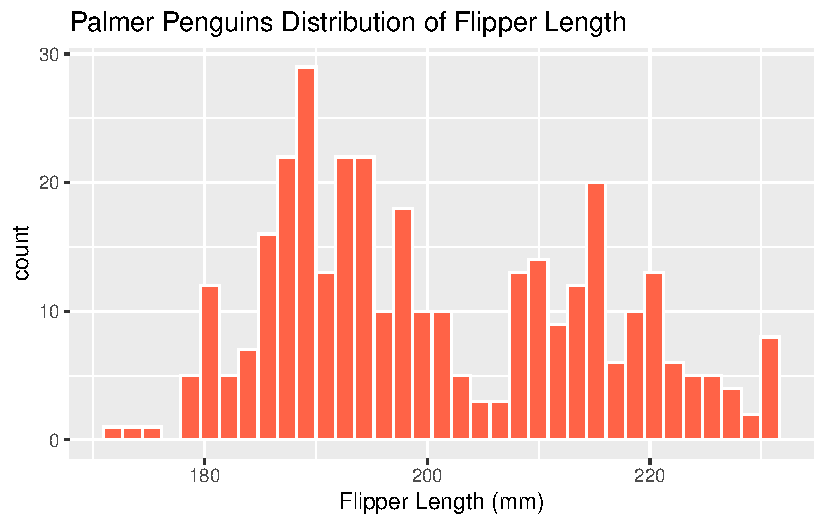
\includegraphics{04-content_files/figure-pdf/unnamed-chunk-8-1.pdf}

}

\end{figure}

\end{tcolorbox}

\begin{tcolorbox}[enhanced jigsaw, breakable, colback=white, bottomrule=.15mm, leftrule=.75mm, colframe=quarto-callout-note-color-frame, arc=.35mm, rightrule=.15mm, toprule=.15mm, left=2mm, opacityback=0]

\begin{itemize}
\item
  Faceting is used to make the same plot for different subgroups of the
  dataset.
\item
  This is useful for comparing the same variable across different
  subgroups in the dataset.
\item
  \texttt{facet\_wrap(\textasciitilde{}var)} can be added on to ANY plot
  type (scatterplot, linegraph, histogram, boxplot, barplot)
\end{itemize}

\begin{Shaded}
\begin{Highlighting}[]
\InformationTok{\textasciigrave{}\textasciigrave{}\textasciigrave{}\{r faceting\}}

\FunctionTok{ggplot}\NormalTok{(penguins, }\FunctionTok{aes}\NormalTok{(}\AttributeTok{x=}\NormalTok{flipper\_length\_mm)) }\SpecialCharTok{+}
    \FunctionTok{geom\_histogram}\NormalTok{(}\AttributeTok{color =} \StringTok{"white"}\NormalTok{, }\AttributeTok{fill =} \StringTok{"tomato1"}\NormalTok{, }\AttributeTok{bins =} \DecValTok{11}\NormalTok{) }\SpecialCharTok{+}
    \FunctionTok{facet\_wrap}\NormalTok{(}\SpecialCharTok{\textasciitilde{}}\NormalTok{ species)}
\InformationTok{\textasciigrave{}\textasciigrave{}\textasciigrave{}}
\end{Highlighting}
\end{Shaded}

\begin{figure}[H]

{\centering 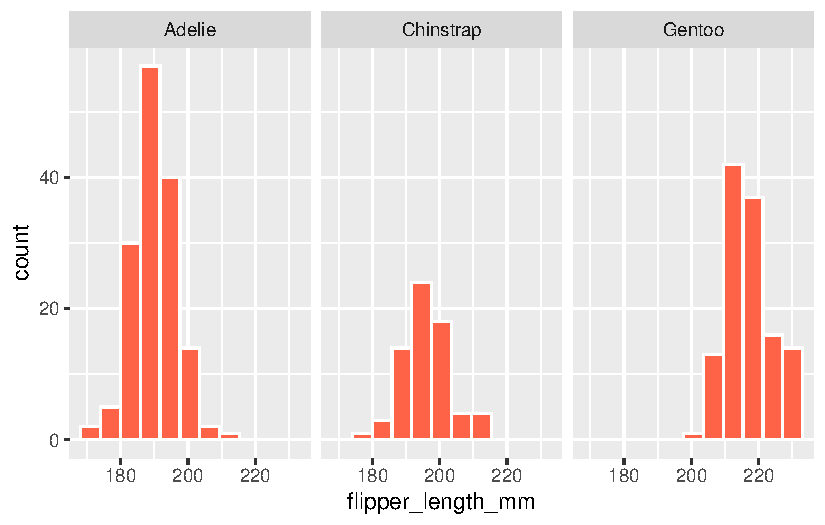
\includegraphics{04-content_files/figure-pdf/faceting-1.pdf}

}

\end{figure}

\end{tcolorbox}

\begin{tcolorbox}[enhanced jigsaw, breakable, colback=white, bottomrule=.15mm, leftrule=.75mm, colframe=quarto-callout-important-color-frame, arc=.35mm, rightrule=.15mm, toprule=.15mm, left=2mm, opacityback=0]

Which is correct?

\begin{itemize}
\tightlist
\item
  b and d
\item
  aes() is for variables! Since ``white'' is not a variable it does not
  go in the aes().
\end{itemize}


\includegraphics[width=\textwidth,height=0.5in]{images/images_lecture/participate_icon.png}

\end{tcolorbox}

\begin{tcolorbox}[enhanced jigsaw, breakable, colback=white, bottomrule=.15mm, leftrule=.75mm, colframe=quarto-callout-note-color-frame, arc=.35mm, rightrule=.15mm, toprule=.15mm, left=2mm, opacityback=0]

Which of the following are correct?

\begin{verbatim}
a)  
\end{verbatim}

\begin{Shaded}
\begin{Highlighting}[]
\InformationTok{\textasciigrave{}\textasciigrave{}\textasciigrave{}\{r\}}
\CommentTok{\#| eval: false}
\FunctionTok{ggplot}\NormalTok{(penguins, }\FunctionTok{aes}\NormalTok{(}\AttributeTok{x=}\NormalTok{flipper\_length\_mm)) }\SpecialCharTok{+}
  \FunctionTok{geom\_histogram}\NormalTok{(}\FunctionTok{aes}\NormalTok{(}\AttributeTok{color =} \StringTok{"white"}\NormalTok{))}
\InformationTok{\textasciigrave{}\textasciigrave{}\textasciigrave{}}
\end{Highlighting}
\end{Shaded}

\begin{verbatim}
b)  
\end{verbatim}

\begin{Shaded}
\begin{Highlighting}[]
\InformationTok{\textasciigrave{}\textasciigrave{}\textasciigrave{}\{r\}}
\CommentTok{\#| eval: false}
\FunctionTok{ggplot}\NormalTok{(penguins, }\FunctionTok{aes}\NormalTok{(}\AttributeTok{x=}\NormalTok{flipper\_length\_mm)) }\SpecialCharTok{+}
  \FunctionTok{geom\_histogram}\NormalTok{(}\AttributeTok{color =} \StringTok{"white"}\NormalTok{)}
\InformationTok{\textasciigrave{}\textasciigrave{}\textasciigrave{}}
\end{Highlighting}
\end{Shaded}

\begin{verbatim}
c)  
\end{verbatim}

\begin{Shaded}
\begin{Highlighting}[]
\InformationTok{\textasciigrave{}\textasciigrave{}\textasciigrave{}\{r\}}
\CommentTok{\#| eval: false}
\FunctionTok{ggplot}\NormalTok{(penguins) }\SpecialCharTok{+}
  \FunctionTok{geom\_histogram}\NormalTok{(}\AttributeTok{x =}\NormalTok{ flipper\_length\_mm, }\AttributeTok{color =} \StringTok{"white"}\NormalTok{)}
\InformationTok{\textasciigrave{}\textasciigrave{}\textasciigrave{}}
\end{Highlighting}
\end{Shaded}

\begin{verbatim}
d)  
\end{verbatim}

\begin{Shaded}
\begin{Highlighting}[]
\InformationTok{\textasciigrave{}\textasciigrave{}\textasciigrave{}\{r\}}
\CommentTok{\#| eval: false}
\FunctionTok{ggplot}\NormalTok{(penguins) }\SpecialCharTok{+}
  \FunctionTok{geom\_histogram}\NormalTok{(}\FunctionTok{aes}\NormalTok{(}\AttributeTok{x =}\NormalTok{ flipper\_length\_mm) , }\AttributeTok{color =} \StringTok{"white"}\NormalTok{)}
\InformationTok{\textasciigrave{}\textasciigrave{}\textasciigrave{}}
\end{Highlighting}
\end{Shaded}

\end{tcolorbox}

\begin{tcolorbox}[enhanced jigsaw, breakable, colback=white, bottomrule=.15mm, leftrule=.75mm, colframe=quarto-callout-note-color-frame, arc=.35mm, rightrule=.15mm, toprule=.15mm, left=2mm, opacityback=0]

\href{https://en.wikipedia.org/wiki/Histogram\#Number_of_bins_and_width}{Wikipedia
bin size info}

Helpful guidelines:

\begin{itemize}
\item
  Larger number of observations generally correspond to larger number of
  bins needed.
\item
  You will generally need to test \textbf{several} different number of
  bins to learn about the data and find an appropriate value.
\item
  Sturges Rule of Thumb for unimodal symmetric distributions: bins = 1 +
  3.322*log(n)
\item
  Sturge's rule is not great if the data is severely skewed,
  multi-modal, or for an extremely large number of observations. But it
  could give you a starting place and then you will want to increase the
  number of bins until you can properly see the shape.
\end{itemize}

\end{tcolorbox}

\hypertarget{activity-solution-2}{%
\section*{Activity Solution}\label{activity-solution-2}}
\addcontentsline{toc}{section}{Activity Solution}

Need to add. See RStudio Cloud TA Solutions for now.

\hypertarget{homework-3}{%
\section*{Homework}\label{homework-3}}
\addcontentsline{toc}{section}{Homework}

\begin{itemize}
\item
  Complete and submit Activity 03
\item
  Read Sections 2.7 - 2.9 of the book
\item
  Complete and submit Reading Check 04\_ggplot3
\end{itemize}

\bookmarksetup{startatroot}

\hypertarget{day-05}{%
\chapter*{Day 05}\label{day-05}}
\addcontentsline{toc}{chapter}{Day 05}

Today's lesson covers
\href{https://nustat.github.io/intro-stat-ds/2-viz.html\#boxplots}{Section
2.7 - 2.9} and focuses on making boxplots and barplots with
\texttt{ggplot()}.

\begin{tcolorbox}[enhanced jigsaw, toptitle=1mm, colback=white, arc=.35mm, rightrule=.15mm, titlerule=0mm, left=2mm, breakable, bottomtitle=1mm, bottomrule=.15mm, leftrule=.75mm, title={Agenda}, colframe=quarto-callout-note-color-frame, opacitybacktitle=0.6, toprule=.15mm, colbacktitle=quarto-callout-note-color!10!white, coltitle=black, opacityback=0]
\textasciitilde{} 15 min Slide deck

\textasciitilde{} 25 min Students work on Activity 02

\textasciitilde{} 10 min Work through a select problem in detail from
the activity as a class
\end{tcolorbox}

\hypertarget{slide-deck-4}{%
\section*{Slide Deck}\label{slide-deck-4}}
\addcontentsline{toc}{section}{Slide Deck}

\begin{tcolorbox}[enhanced jigsaw, breakable, colback=white, bottomrule=.15mm, leftrule=.75mm, colframe=quarto-callout-note-color-frame, arc=.35mm, rightrule=.15mm, toprule=.15mm, left=2mm, opacityback=0]

\begin{enumerate}
\def\labelenumi{\arabic{enumi}.}
\tightlist
\item
  Create a boxplot
\item
  Create a barplot
\item
  Properly describe a boxplot and barplot
\item
  Display barplots in various ways by category
\end{enumerate}


\includegraphics[width=\textwidth,height=1in]{images/images_horst/r_first_then.png}
Artwork by @allison\_horst

\end{tcolorbox}

\begin{tcolorbox}[enhanced jigsaw, breakable, colback=white, bottomrule=.15mm, leftrule=.75mm, colframe=quarto-callout-note-color-frame, arc=.35mm, rightrule=.15mm, toprule=.15mm, left=2mm, opacityback=0]

\begin{itemize}
\item
  A boxplot is used to visualize the \textbf{distribution} of a single
  \textbf{numerical} variable.
\item
  Grouped boxplots are particularly useful for comparing the
  distribution of a numerical variable across a \textbf{categorical}
  variable. ie: shows the relationship between a numerical and a
  categorical variable.
\end{itemize}

\textbf{Boxplot syntax in R:}

\begin{Shaded}
\begin{Highlighting}[]
\FunctionTok{ggplot}\NormalTok{(}\AttributeTok{data=}\NormalTok{ my\_data, }\FunctionTok{aes}\NormalTok{(}\AttributeTok{x =}\NormalTok{ (optional categorical variable),  }\AttributeTok{y =}\NormalTok{ var1)) }\SpecialCharTok{+}
  \FunctionTok{geom\_boxplot}\NormalTok{()}
\end{Highlighting}
\end{Shaded}

If you switch x and y, it will just change the orientation of the
boxplot (personal preference).

\end{tcolorbox}

\begin{tcolorbox}[enhanced jigsaw, breakable, colback=white, bottomrule=.15mm, leftrule=.75mm, colframe=quarto-callout-note-color-frame, arc=.35mm, rightrule=.15mm, toprule=.15mm, left=2mm, opacityback=0]

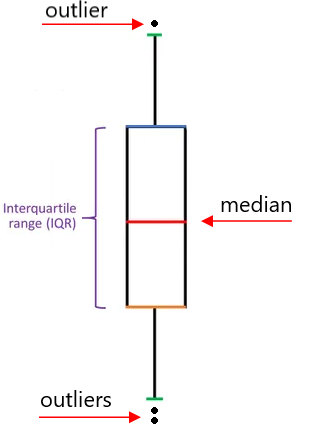
\includegraphics[width=\textwidth,height=2in]{images/images_lecture/box_plot.png}

There are 3 things that we typically focus on and describe/compare when
inspecting a boxplot:

\begin{itemize}
\tightlist
\item
  center
\item
  spread
\item
  shape and outliers
\end{itemize}

\end{tcolorbox}

\begin{tcolorbox}[enhanced jigsaw, breakable, colback=white, bottomrule=.15mm, leftrule=.75mm, colframe=quarto-callout-important-color-frame, arc=.35mm, rightrule=.15mm, toprule=.15mm, left=2mm, opacityback=0]

Is \texttt{Survived} a categorical or numerical variable?

\begin{itemize}
\tightlist
\item
  It should be categorical even though it is coded as numerical ``dbl''
\end{itemize}


\includegraphics[width=\textwidth,height=0.5in]{images/images_lecture/participate_icon.png}

\end{tcolorbox}

\begin{tcolorbox}[enhanced jigsaw, breakable, colback=white, bottomrule=.15mm, leftrule=.75mm, colframe=quarto-callout-note-color-frame, arc=.35mm, rightrule=.15mm, toprule=.15mm, left=2mm, opacityback=0]
Consider the \texttt{titanic} dataset, which contains information about
passengers on the titanic. If a passenger survived, then the variable
\texttt{Survived\ =\ 1}.

\begin{Shaded}
\begin{Highlighting}[]
\InformationTok{\textasciigrave{}\textasciigrave{}\textasciigrave{}\{r\}}

\NormalTok{titanic }\SpecialCharTok{\%\textgreater{}\%} 
  \FunctionTok{select}\NormalTok{(PassengerId, Survived, Sex) }\SpecialCharTok{\%\textgreater{}\%}
  \FunctionTok{glimpse}\NormalTok{()}
\InformationTok{\textasciigrave{}\textasciigrave{}\textasciigrave{}}
\end{Highlighting}
\end{Shaded}

\begin{verbatim}
Rows: 418
Columns: 3
$ PassengerId <dbl> 892, 893, 894, 895, 896, 897, 898, 899, 900, 901, 902, 903~
$ Survived    <dbl> 0, 1, 0, 0, 1, 0, 1, 0, 1, 0, 0, 0, 1, 0, 1, 1, 0, 0, 1, 1~
$ Sex         <chr> "male", "female", "male", "male", "female", "male", "femal~
\end{verbatim}

Is \texttt{Survived} a categorical or numerical variable?

\texttt{R} will read in numerical columns as ``numbers'' even though
these numbers are supposed to represent ``categories''.

To fix this we need to use the \texttt{factor()} function.

Typing \texttt{factor(Survived)} would turn the variable into a
``factor''.
\end{tcolorbox}

\begin{tcolorbox}[enhanced jigsaw, breakable, colback=white, bottomrule=.15mm, leftrule=.75mm, colframe=quarto-callout-note-color-frame, arc=.35mm, rightrule=.15mm, toprule=.15mm, left=2mm, opacityback=0]

A barplot is used to visualize the distribution (frequencies) of a
single categorical variable.

\begin{itemize}
\item
  \texttt{geom\_bar()} is used when we have the raw data and counting
  how many observations are in each category has to be done (list not
  yet counted).
\item
  \texttt{geom\_col()} is used when we directly have counts of each
  category in our dataset (pre-counted).
\end{itemize}

\textbf{Barplot syntax in R:}

\begin{Shaded}
\begin{Highlighting}[]
\FunctionTok{ggplot}\NormalTok{(}\AttributeTok{data=}\NormalTok{ my\_data, }\FunctionTok{aes}\NormalTok{(}\AttributeTok{x =}\NormalTok{ var1)) }\SpecialCharTok{+}
  \FunctionTok{geom\_bar}\NormalTok{()}
\end{Highlighting}
\end{Shaded}

\end{tcolorbox}

\begin{tcolorbox}[enhanced jigsaw, breakable, colback=white, bottomrule=.15mm, leftrule=.75mm, colframe=quarto-callout-note-color-frame, arc=.35mm, rightrule=.15mm, toprule=.15mm, left=2mm, opacityback=0]

When describing a barplot we look for\ldots{}

\begin{itemize}
\tightlist
\item
  Disparities in the height of the bars.
\item
  Bar with the most observations.
\item
  Bar with the least observations.
\item
  If all the bars are about equal height, then the distribution is
  uniform.
\end{itemize}

\end{tcolorbox}

\begin{tcolorbox}[enhanced jigsaw, breakable, colback=white, bottomrule=.15mm, leftrule=.75mm, colframe=quarto-callout-important-color-frame, arc=.35mm, rightrule=.15mm, toprule=.15mm, left=2mm, opacityback=0]

Are we using \texttt{geom\_bar()} or \texttt{geom\_col()}?

\begin{itemize}
\tightlist
\item
  \texttt{geom\_bar()}
\end{itemize}


\includegraphics[width=\textwidth,height=0.5in]{images/images_lecture/participate_icon.png}

\end{tcolorbox}

\begin{tcolorbox}[enhanced jigsaw, breakable, colback=white, bottomrule=.15mm, leftrule=.75mm, colframe=quarto-callout-note-color-frame, arc=.35mm, rightrule=.15mm, toprule=.15mm, left=2mm, opacityback=0]

Consider the Palmer Penguins dataset.

\begin{Shaded}
\begin{Highlighting}[]
\InformationTok{\textasciigrave{}\textasciigrave{}\textasciigrave{}\{r\}}

\FunctionTok{library}\NormalTok{(palmerpenguins)}
\FunctionTok{head}\NormalTok{(penguins)}
\InformationTok{\textasciigrave{}\textasciigrave{}\textasciigrave{}}
\end{Highlighting}
\end{Shaded}

\begin{verbatim}
# A tibble: 6 x 8
  species island    bill_length_mm bill_depth_mm flipper_l~1 body_~2 sex    year
  <fct>   <fct>              <dbl>         <dbl>       <int>   <int> <fct> <int>
1 Adelie  Torgersen           39.1          18.7         181    3750 male   2007
2 Adelie  Torgersen           39.5          17.4         186    3800 fema~  2007
3 Adelie  Torgersen           40.3          18           195    3250 fema~  2007
4 Adelie  Torgersen           NA            NA            NA      NA <NA>   2007
5 Adelie  Torgersen           36.7          19.3         193    3450 fema~  2007
6 Adelie  Torgersen           39.3          20.6         190    3650 male   2007
# ... with abbreviated variable names 1: flipper_length_mm, 2: body_mass_g
\end{verbatim}

We are interested in plotting the distribution of \texttt{species}.

Are we using \texttt{geom\_bar()} or \texttt{geom\_col()}?

What would pre-counted data look like?

\hypertarget{data-3}{%
\subsubsection*{Data}\label{data-3}}
\addcontentsline{toc}{subsubsection}{Data}

\begin{Shaded}
\begin{Highlighting}[]
\InformationTok{\textasciigrave{}\textasciigrave{}\textasciigrave{}\{r\}}

\NormalTok{penguins\_counted}
\InformationTok{\textasciigrave{}\textasciigrave{}\textasciigrave{}}
\end{Highlighting}
\end{Shaded}

\begin{verbatim}
# A tibble: 3 x 2
  species       n
  <fct>     <int>
1 Adelie      152
2 Chinstrap    68
3 Gentoo      124
\end{verbatim}

\hypertarget{code}{%
\subsubsection*{Code}\label{code}}
\addcontentsline{toc}{subsubsection}{Code}

\begin{Shaded}
\begin{Highlighting}[]
\InformationTok{\textasciigrave{}\textasciigrave{}\textasciigrave{}\{r\}}

\NormalTok{penguins\_counted }\OtherTok{\textless{}{-}}\NormalTok{ penguins }\SpecialCharTok{\%\textgreater{}\%} 
  \FunctionTok{count}\NormalTok{(species)}
\InformationTok{\textasciigrave{}\textasciigrave{}\textasciigrave{}}
\end{Highlighting}
\end{Shaded}

\end{tcolorbox}

\begin{tcolorbox}[enhanced jigsaw, toptitle=1mm, colback=white, arc=.35mm, rightrule=.15mm, titlerule=0mm, left=2mm, breakable, bottomtitle=1mm, bottomrule=.15mm, leftrule=.75mm, title={Teaching note:}, colframe=quarto-callout-important-color-frame, opacitybacktitle=0.6, toprule=.15mm, colbacktitle=quarto-callout-important-color!10!white, coltitle=black, opacityback=0]

\begin{itemize}
\tightlist
\item
  stacked: best if you are interested in overall counts but difficult to
  visually see if there is a difference between categories because of
  the \textbf{different counts}
\item
  proportion: best if you are interested in the \textbf{rate} within
  each category. Not concerned with counts.
\item
  side-by-side: best if you want to see differences between categories
  but still want to see the count discrepancies between the main
  category
\end{itemize}

\end{tcolorbox}

\begin{tcolorbox}[enhanced jigsaw, breakable, colback=white, bottomrule=.15mm, leftrule=.75mm, colframe=quarto-callout-note-color-frame, arc=.35mm, rightrule=.15mm, toprule=.15mm, left=2mm, opacityback=0]

What if we want to visualize the distribution of \texttt{sex} in each of
the \texttt{species}. There are 4 main ways to visualize multiple levels
within a categorical data:

\begin{Shaded}
\begin{Highlighting}[]
\FunctionTok{ggplot}\NormalTok{(}\AttributeTok{data=}\NormalTok{penguins, }\FunctionTok{aes}\NormalTok{(}\AttributeTok{x =}\NormalTok{ species, }\AttributeTok{fill =}\NormalTok{ sex)) }\SpecialCharTok{+}
  \FunctionTok{geom\_bar}\NormalTok{()}
\end{Highlighting}
\end{Shaded}

\begin{figure}[H]

{\centering 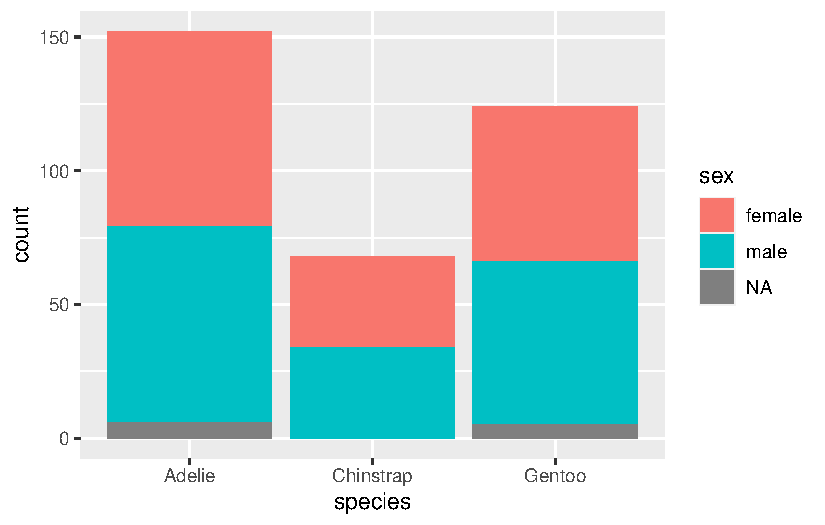
\includegraphics[width=0.5\textwidth,height=\textheight]{05-content_files/figure-pdf/cat-barplot-1.pdf}

}

\end{figure}

\begin{Shaded}
\begin{Highlighting}[]
\FunctionTok{ggplot}\NormalTok{(}\AttributeTok{data=}\NormalTok{penguins, }\FunctionTok{aes}\NormalTok{(}\AttributeTok{x =}\NormalTok{ species, }\AttributeTok{fill =}\NormalTok{ sex)) }\SpecialCharTok{+}
  \FunctionTok{geom\_bar}\NormalTok{(}\AttributeTok{position =} \StringTok{"fill"}\NormalTok{) }\SpecialCharTok{+}
  \FunctionTok{ylab}\NormalTok{(}\StringTok{"proportion"}\NormalTok{)}
\end{Highlighting}
\end{Shaded}

\begin{figure}[H]

{\centering 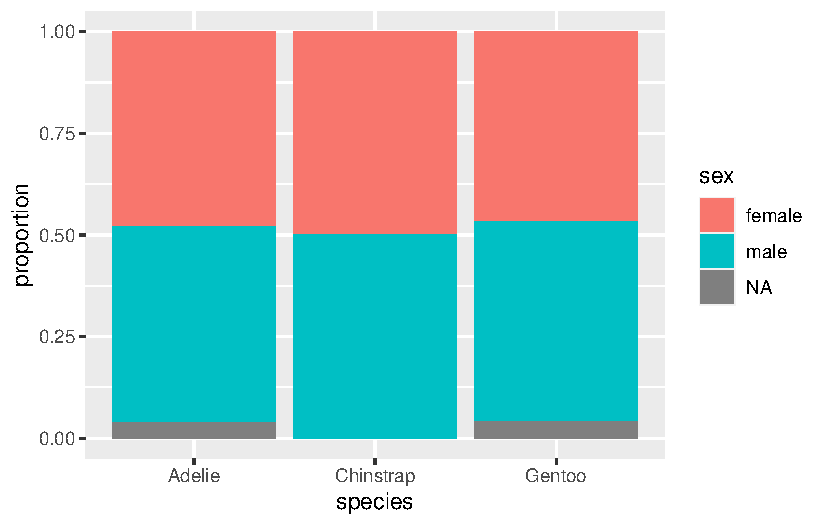
\includegraphics[width=0.5\textwidth,height=\textheight]{05-content_files/figure-pdf/proportion-barplot-1.pdf}

}

\end{figure}

\begin{Shaded}
\begin{Highlighting}[]
\FunctionTok{ggplot}\NormalTok{(}\AttributeTok{data=}\NormalTok{penguins, }\FunctionTok{aes}\NormalTok{(}\AttributeTok{x =}\NormalTok{ species, }\AttributeTok{fill =}\NormalTok{ sex)) }\SpecialCharTok{+}
  \FunctionTok{geom\_bar}\NormalTok{(}\AttributeTok{position =} \StringTok{"dodge"}\NormalTok{)}
\end{Highlighting}
\end{Shaded}

\begin{figure}[H]

{\centering 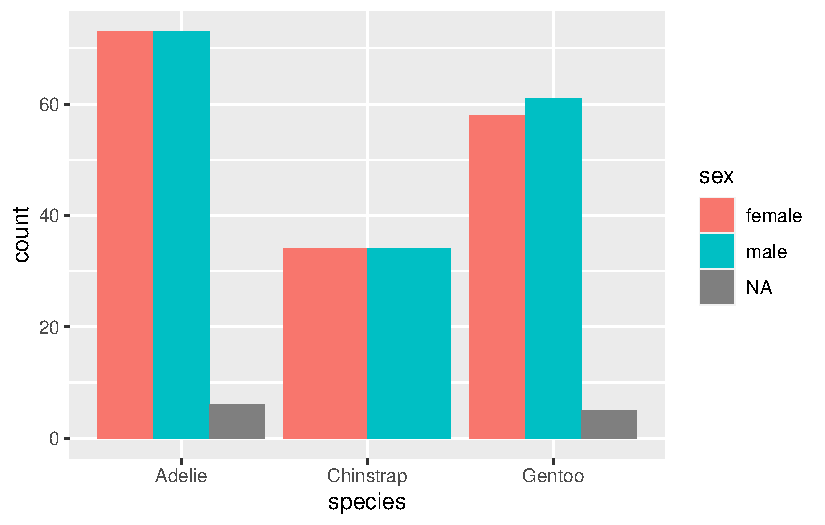
\includegraphics[width=0.5\textwidth,height=\textheight]{05-content_files/figure-pdf/side-by-side-barplot-1.pdf}

}

\end{figure}

\begin{Shaded}
\begin{Highlighting}[]
\FunctionTok{ggplot}\NormalTok{(}\AttributeTok{data=}\NormalTok{penguins, }\FunctionTok{aes}\NormalTok{(}\AttributeTok{x =}\NormalTok{ species))}\SpecialCharTok{+}
  \FunctionTok{geom\_bar}\NormalTok{() }\SpecialCharTok{+}
  \FunctionTok{facet\_wrap}\NormalTok{(}\SpecialCharTok{\textasciitilde{}}\NormalTok{ sex)}
\end{Highlighting}
\end{Shaded}

\begin{figure}[H]

{\centering 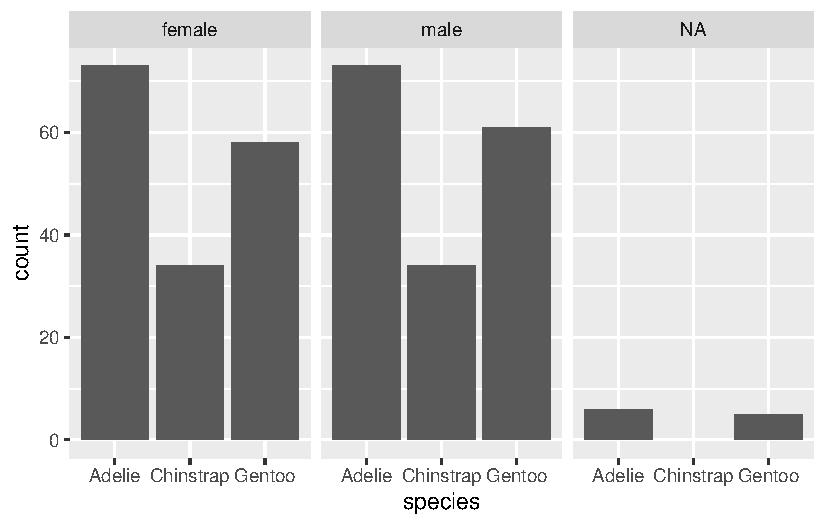
\includegraphics[width=0.5\textwidth,height=\textheight]{05-content_files/figure-pdf/faceted-barplot-1.pdf}

}

\end{figure}

\end{tcolorbox}

\begin{tcolorbox}[enhanced jigsaw, breakable, colback=white, bottomrule=.15mm, leftrule=.75mm, colframe=quarto-callout-note-color-frame, arc=.35mm, rightrule=.15mm, toprule=.15mm, left=2mm, opacityback=0]

\textbf{``factor'' vs ``character'' variable}

\begin{itemize}
\tightlist
\item
  factor has predefined levels and the observation must be one of those
  levels (limited response options).
\item
  character can take on any string value (think open response options)
\item
  \href{https://www.stat.berkeley.edu/~s133/factors.html}{Factors in R}
\end{itemize}

\end{tcolorbox}

\hypertarget{activity-solution-3}{%
\section*{Activity Solution}\label{activity-solution-3}}
\addcontentsline{toc}{section}{Activity Solution}

Need to add. See RStudio Cloud TA Solutions for now.

\hypertarget{homework-4}{%
\section*{Homework}\label{homework-4}}
\addcontentsline{toc}{section}{Homework}

\begin{itemize}
\item
  Complete and submit Activity 04
\item
  Read Sections 3.0 - 3.3 of the book
\item
  Complete and submit Reading Check 05\_wrangling1
\end{itemize}

\bookmarksetup{startatroot}

\hypertarget{references}{%
\chapter*{References}\label{references}}
\addcontentsline{toc}{chapter}{References}

\hypertarget{refs}{}
\begin{CSLReferences}{0}{0}
\end{CSLReferences}



\end{document}
